%%%%%%%%%%%%%%%%%%%%%%%%%%%%%%%%%%%%%%%%%
% Masters/Doctoral Thesis
% LaTeX Template
% Version 2.5 (27/8/17)
%
% This template was downloaded from:
% http://www.LaTeXTemplates.com
%
% Version 2.x major modifications by:
% Vel (vel@latextemplates.com)
%
% This template is based on a template by:
% Steve Gunn (http://users.ecs.soton.ac.uk/srg/softwaretools/document/templates/)
% Sunil Patel (http://www.sunilpatel.co.uk/thesis-template/)
%
% Template license:
% CC BY-NC-SA 3.0 (http://creativecommons.org/licenses/by-nc-sa/3.0/)
%
%%%%%%%%%%%%%%%%%%%%%%%%%%%%%%%%%%%%%%%%%

%----------------------------------------------------------------------------------------
%	PACKAGES AND OTHER DOCUMENT CONFIGURATIONS
%----------------------------------------------------------------------------------------

% Pages (from the internal page numbering) to be printed in color - 3, 4, 5, 11, 12, 13, 14, 17, 18, 20, 21, 23, 25, 27.

\documentclass[
hidelinks,
12pt, % The default document font size, options: 10pt, 11pt, 12pt
oneside, % Two side (alternating margins) for binding by default, uncomment to switch to one side
english, % ngerman for German
doublespacing, % Single line spacing, alternatives: onehalfspacing or singlespacing
%draft, % Uncomment to enable draft mode (no pictures, no links, overfull hboxes indicated)
%nolistspacing, % If the document is onehalfspacing or doublespacing, uncomment this to set spacing in lists to single
%liststotoc, % Uncomment to add the list of figures/tables/etc to the table of contents
%toctotoc, % Uncomment to add the main table of contents to the table of contents
%parskip, % Uncomment to add space between paragraphs
%nohyperref, % Uncomment to not load the hyperref package
headsepline, % Uncomment to get a line under the header
%chapterinoneline, % Uncomment to place the chapter title next to the number on one line
%consistentlayout, % Uncomment to change the layout of the declaration, abstract and acknowledgements pages to match the default layout
]{MastersDoctoralThesis} % The class file specifying the document structure

\usepackage[utf8]{inputenc} % Required for inputting international characters
\usepackage[T1]{fontenc} % Output font encoding for international characters
% \usepackage{subcaption}
\usepackage{mathpazo} % Use the Palatino font by default
\usepackage{booktabs}
\usepackage{amssymb}
\usepackage{colortbl}
\usepackage[final]{pdfpages}
\usepackage{xcolor}
\usepackage{balance}
\usepackage{epigraph}
\usepackage{alltt} % for code snippet
\usepackage{listings}
\usepackage{hyperref}
\usepackage{amsmath}
\usepackage{macros}
\usepackage{mathtools}
\usepackage{float}
\usepackage{newtxmath}
\usepackage{polski}
\usepackage{bbm}
\usepackage{tikz-cd}
\usepackage{flowchart}
\usepackage{tabularx}
\usepackage{array}
\setlength\extrarowheight{2pt}
\usepackage[mathscr]{euscript}
\usetikzlibrary{
  shapes,
  arrows.meta, % supersedes arrows
  calc,automata,positioning,fit,quotes}
  \tikzset{
  line/.style={draw, -Latex}
}
\tikzstyle{arrow} = [thick,->,>=stealth]
\DeclareMathOperator{\Cech}{\check{C}}
\usepackage[backend=bibtex,style=authoryear,natbib=true]{biblatex} % Use the bibtex backend with the authoryear citation style (which resembles APA)
%\usepackage[backend=bibtex,style=authoryear,natbib=true,backref=true]{biblatex} % use this line instead of the previous one if you want to use back references
\usepackage{caption}
\usepackage{subcaption}
\captionsetup{font=normalsize,labelfont={bf,sf}}
\captionsetup[subfigure]{font=scriptsize,labelfont=scriptsize}
% \usepackage{subfig, graphicx}

\addbibresource{biblio.bib} % The filename of the bibliography


\usepackage[autostyle=true]{csquotes} % Required to generate language-dependent quotes in the bibliography

%----------------------------------------------------------------------------------------
%	MARGIN SETTINGS
%----------------------------------------------------------------------------------------

\geometry{
	paper=a4paper, % Change to letterpaper for US letter
	inner=4.0cm, % Inner margin
	outer=3.0cm, % Outer margin
	bindingoffset=.5cm, % Binding offset
	top=2.5cm, % Top margin
	bottom=2.5cm, % Bottom margin
	head=23.99748pt,
	%showframe, % Uncomment to show how the type block is set on the page
}

%----------------------------------------------------------------------------------------
%	THESIS INFORMATION
%----------------------------------------------------------------------------------------

\thesistitle{$p$-Wasserstein Distance between High-dimensional Point Clouds \\ via Persistent Homology} % Your thesis title, this is used in the title and abstract, print it elsewhere with \ttitle
\supervisor{Dr/Pr. FirstName \textsc{LastName}} % Your supervisor's name, this is used in the title page, print it elsewhere with \supname
\examiner{Dr/Pr. FirstName \textsc{LastName}} % Your examiner's name, this is not currently used anywhere in the template, print it elsewhere with \examname
\degree{B.Sc (Hons)} % Your degree name, this is used in the title page and abstract, print it elsewhere with \degreename
\author{\textsc{Zhang} Liu} % Your name, this is used in the title page and abstract, print it elsewhere with \authorname
\addresses{} % Your address, this is not currently used anywhere in the template, print it elsewhere with \addressname

\subject{Mathematical, Computational and Statistical Sciences} % Your subject area, this is not currently used anywhere in the template, print it elsewhere with \subjectname
\keywords{applied topology, persistent homology, Wasserstein distance, dimensionality reduction, diffusion map} % Keywords for your thesis, this is not currently used anywhere in the template, print it elsewhere with \keywordnames
\university{\href{https://www.nus.edu.sg/}{National University of Singapore}} % Your university's name and URL, this is used in the title page and abstract, print it elsewhere with \univname
\department{{}} % Your department's name and URL, this is used in the title page and abstract, print it elsewhere with \deptname
\group{{}} % Your research group's name and URL, this is used in the title page, print it elsewhere with \groupname
\faculty{{}} % Your faculty's name and URL, this is used in the title page and abstract, print it elsewhere with \facname

\AtBeginDocument{
% \hypersetup{colorlinks=false}
\hypersetup{pdftitle=\ttitle} % Set the PDF's title to your title
\hypersetup{pdfauthor=\authorname} % Set the PDF's author to your name
\hypersetup{pdfkeywords=\keywordnames} % Set the PDF's keywords to your keywords
\hypersetup{hypertexnames=true}
}

\begin{document}

\frontmatter 
\pagestyle{plain} 

\begin{titlepage}
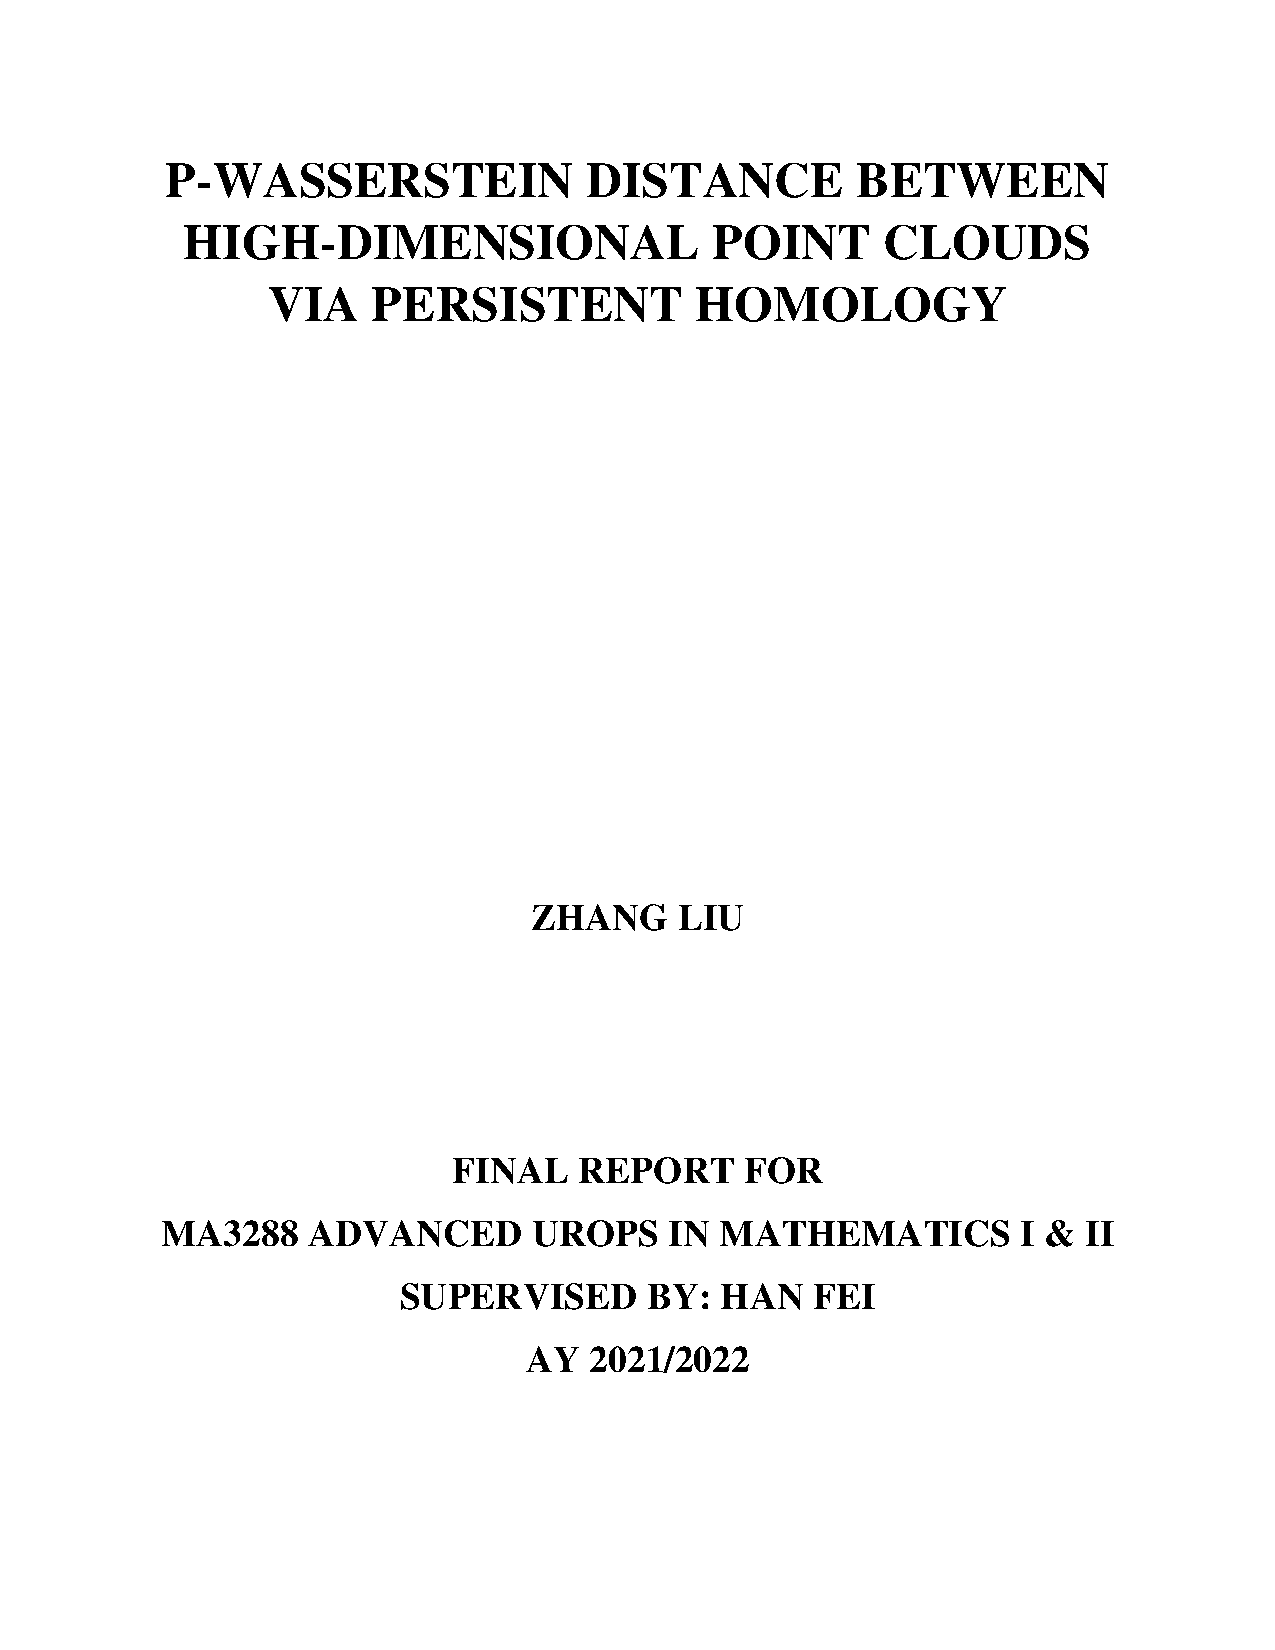
\includepdf[pages=-,pagecommand={},width=\textwidth]{titlepage.pdf}

\end{titlepage}

\begin{acknowledgements}
\addchaptertocentry{\acknowledgementname} % Add the acknowledgements to the table of contents
    I would like to thank my mentor Prof.~Han Fei for his continual support throughout the project. There have been ups and downs in this project, but Prof.~Han Fei has helped me stay flexible and keep a keen spirit for learning and discovery. I am also grateful for support from my family and friends.
\end{acknowledgements}

\begin{abstract}
\addchaptertocentry{\abstractname} % Add the abstract to the table of contents
\textbf{Key words: \keywordnames}

Topological Data Analysis (TDA) is a recent field that emerged from various works in applied (algebraic) topology and computational geometry. 
The aim of TDA is to extract and analyze relevant topological and geometric features of real-world data, which are often high-dimensional and have complex underlying geometric structures. 

Our project is motivated by the question: how can high-dimensional point clouds be compared based on their topological structures? 
To this end, we proposed an approach to compare point clouds based on the $p$-Wasserstein distance of their topological fingerprints. 
We illustrated the approach with a concrete application in studying the neural population responses to different stimuli, each of which is represented as a high-dimensional point cloud. Our approach allowed us to quantify the pairwise similarity of the neural population responses in terms of their topological structures.
Using this approach, we also compared the topological structure of the point cloud associated with each neural population response with that of synthetic data sampled from $2$-sphere and torus.
\end{abstract}

\tableofcontents


\mainmatter 
\pagestyle{thesis}

\chapter{Introduction} 
\label{Chapter1-intro} 

\section{Background}
Topological Data Analysis (TDA) is a recent field that emerged from various works in applied (algebraic) topology and computational geometry during the first decade of the century. It started as a field with the foundational works of (\cite{edelsbrunner_topological_2002}) and (\cite{Zom2005a}) and was popularized by (\cite{carlsson_topology_2009}). The aim of TDA is to extract, analyze and make use of the topological and geometric structures underlying data. These data are usually represented as point clouds in Euclidean or more general metric spaces and are often high-dimensional. (\cite{chazal_introduction_2021})

\section{Aim and Significance}
Our project is motivated by the following question: how can high-dimensional point clouds be compared based on their topological structures? To this end, we studied the theory of persistent homology, dimensionality reduction, and various distance metrics useful for high-dimensional data analysis. Further, we proposed an approach to compare point clouds based on the $p$-Wasserstein distance of their topological fingerprints. We illustrated the approach with a concrete application using neural spiking data from lab experiments. The code for this project can be found in the GitHub repository \footnote{https://github.com/zhang-liu-official/UROPS-2021-Topological-Data-Analysis} and Appendix \ref{AppendixA}.

The topological methods used in this project provide a new perspective to compare data point clouds as shapes. Topological features capture the global structure of the data, which is especially important in applications where the notion of connectedness and clusters are salient.


\section{Prior works applying topological methods in neuroscience}

The first work that applied topological methods in neuroscience is (\cite{singh_top_v1_2008}). The authors applied computational topology to analyze neural population activity in the primary visual cortex and concluded that the topological structure of neural population activity is align with the topological structure of a $2$-sphere both when the cortex is spontaneously active and when evoked by natural images.

Following that, there have been many applications of persistent homology in studying the topological structure of neural population activity across different systems. A notable application is (\cite{chaudhuri_intrinsic_2019}), where the authors applied persistent homology to study the the neural population activity from the post-subiculum and anterodorsal thalamus. They showed that the head direction of mice can be decoded from a one-dimensional ring structure. A recent addition in this line of work was by (\cite{beshkov_geodesic-based_2021}). They showed that when using the geodesic distance instead of the Euclidean distance, persistent homology method was able to successfully identify highly non-linear features. They then provided an application using the Neuropixels dataset recorded in mouse visual cortex after stimulation with drifting gratings.

An alternative approach has been taken by several researchers to to use spike train correlation measures to define the ``distance" between two neurons by how similar the firing rates of two neurons are given a stimuli. This was computed this from the neural spiking data. With the spike train correlation measures, they then obtained the so-called neural clique topology. Two notable works are  (\cite{giusti_clique_2015}) and (\cite{bardin_topological_2019}). 

\chapter{Persistent Homology} 
\label{chapter3-homology}

This chapter includes the necessary theoretical background of persistent homology. The main references for this chapter are (\cite{carlsson_topology_2009}) and (\cite{zomorodian_computing_nodate}).

\section{Motivation}

First of all, there are four major advantages for using topological methods to analyze high-dimensional point clouds.

\begin{enumerate}
	\item Topology provides qualitative information which is required for data analysis.
	
	\item Metrics are not theoretically justified. Compared to straightforward geometric methods, Topology is less sensitive to the actual choice of metrics. 
	
	\item Studying geometric objects using Topology does not depend on the coordinates. 
	
	\item Functoriality. This is the most important advantage.
	
	\begin{defn}[Functoriality]
	
		For any topological space X, abelian group $A$, and integer $k\geq 0,$ there is assigned a group $H_k(X,A).$ For any $A$ and $k$, and any continuous map $f: X \to Y,$ there is an induced homomorphism $H_k(f,A): H_k(X,A) \to H_k(Y,A).$ Then \underline{functoriality} refers to the following conditions:
		\begin{itemize}
			\item  $H_k(f\circ g,A): H_k(f,A) \circ H_k(g,A)$
			\item  $H_k(Id_{X};A) = Id_{H_k(X,A)}.$
		\end{itemize}
	\end{defn}
	Functoriality addresses the ambiguities in statistical clustering methods -- in particular the arbitrariness of various threshold choices. We now illustrate how exactly functoriality could be used in questions related to clustering. 
	
	Let $X$ be the full data set and $X_1,X_2$ are the subsamples from the data set. If the set of clusterings $C(X_1), C(X_2), C(X_1 \cup X_2)$ correspond well, then we can conclude that the subsample clusterings correspond to clusterings in the full data set $X$. 
\end{enumerate}

\section{Homotopy} \label{sec:homotopy}

\begin{defn}[Homotopy]

	\underline{Homotopy} is a family of maps $f_t: X \to Y$ where $t \in I$ such that $F: X\times I \to Y$ defined by $F(x,t) \mapsto f_t(x)$ is continuous.
	
	Two maps $f_0, f_1$ are \underline{homotopic} if there exists a homotopy $f_t$ between $f_0$ and $f_1$.  
\end{defn}

% A special case of homotopy is the deformation retraction. 

% \begin{defn}[Deformation retraction]
% 	A \underline{deformation retraction} of $X$ onto a subspace $A$ is a homotopy from the identity map of $X$ to a retraction of $X$ onto $A$, $r: X\to X$ such that $r(X) = A$ and $r|_A = \mathbbm{1}$ (or equivalently, retraction is the map $r: X\to X, r^2 =r$). 
% \end{defn}

% Retraction is the topological analog of projection. To visualize this analogy, we give an example of how some deformation retractions arise from the mapping cylinder.

% \begin{defn}
% 	For a map $f: X\to Y$, the \textit{mapping cylinder} $M_f$ is the quotient space of the disjoint union $(X \times I) \sqcup Y$.
% \end{defn}

\begin{defn}[Homotopy equivalence]

A map $f:X \to Y$ is a \underline{homotopy equivalence} if there is a map $g: Y \to X$ such that 
\begin{itemize}
	\item $f\circ g$ is homotopic to the identity map on $Y$, and
	\item $g\circ f$ is homotopic to $f$.
\end{itemize}

Two spaces $X,Y$ are\textit{ homotopy equivalent} if there exists a homotopy equivalence $f: X \to Y. $
\end{defn}

\begin{thm}
	If $f$ and $g$ are homotopic, then $H_k(f,A) = H_k(g,A).$ 
	
	If $X$ and $Y$ are homotopy equivalent, then $H_k(X,A) \cong H_k(Y,A) $.
	
	Note that if two spaces are homotopy equivalent, then all their Betti numbers (defined in subsequent section) are equal.
\end{thm}
\begin{defn}[Topological space]
    Associated to a simplicial complex $(V, \triangle)$ is a topological space $|(V,\triangle)|$. $|(V,\triangle)|$ may be defined using a bijection $\phi : V \to \{1, 2, \dots,N\}$ as the subspace of $\mathbb{R}^N$ given by the union 
	$$\bigcup_{\sigma \in \triangle} c(\sigma),$$
	where $c(\sigma)$ is the convex hull of the set $\{e_{\phi(s)}\}_{s\in \sigma}$, where $e_i$ denotes the $i$-th standard basis vector.

	 We often use abstract simplicial complexes to approximate topological spaces. For simplicial complexes the homology can be computed using only the linear algebra of finitely generated $\mathbb{Z}$-modules. In particular, for simplicial complexes, homology is algorithmically computable.
\end{defn}	
	
\begin{defn}[Nerve]
	Let $X$ be a topological space, and let $\mathcal{U} = \{U_\alpha\}_{\alpha\in A}$ be any covering of $X$. 
	
	The \underline{nerve} of $\mathcal{U}$, denoted by $N(\mathcal{U})$, will be the abstract simplicial complex with vertex set $A$, and where a family $\{\alpha_0, \dots, \alpha_k\}$ spans a $k$-simplex if and only if $U_{\alpha_0}\cap U_{\alpha_1} \cap \cdots \cap U_{\alpha_k} \neq \emptyset.$
\end{defn}

One reason that this construction is very useful in the following ``Nerve Theorem." This theorem gives the criteria for $N(\mathcal{U})$ to be homotopy equivalent to the underlying topological space $X$.

\begin{thm}[Nerve Theorem]
Suppose that $X$ and $U$ are as above, and suppose that the covering consists of open sets and is numerable. Suppose further that for all $\emptyset \subseteq A,$ we have that $\bigcap_{s\in S} U_s$ is either contractible or empty. Then $N(\mathcal{U})$ is homotopy equivalent to $X$.
\end{thm}
The Nerve Theorem is very important in TDA since it provides a way to encode the topology of continuous spaces into abstract combinatorial structures that are more useful for designing computationally efficient data structures and algorithms.

\section{Simplicial Complexes}

\begin{defn}[Simplicial complex]

	An \underline{abstract simplicial complex} is a pair $(V, \triangle)$, where $V$ is a finite set, and $\triangle$ is a family of non-empty subsets of $V$ such that 
	$$\tau \in \triangle \text{ and }\sigma \subseteq \tau \implies \sigma \in \triangle.$$
	
	$\tau \in \triangle $ is face of $\triangle$. The dimension of a face $\tau$ is $|\tau| - 1.$
	
	(Intuition) A simplicial complex $\triangle$ in $\mathbb{R}^n$ is a collection of simplices in $\mathbb{R}^n$ such that
	\begin{enumerate}
	    \item Every face of a simplex of $\triangle$ is in $\triangle$.
	    \item The intersection of any two simplicies of $\triangle$ is a face of each. 
	\end{enumerate}
\end{defn}

\begin{defn}[Maximal Face]

A face $\tau$ is a \underline{maximal face} of $\triangle$ if there is no face $\sigma$ of $\triangle$ such that $\tau \subsetneq \sigma.$
\begin{itemize}
    \item 0-dimensional faces: vertices
    \item 1-dimensional faces: edges
    \item A simplicial complex of dimension $D \leq 1$ is a simple and loopless graph.
\end{itemize}
\end{defn}

\begin{defn}[k-skeleton]

    A simplicial complex $\triangle_0$ is a subcomplex of $\triangle$ if $\triangle_0 \subseteq \triangle$.
    
    For $k\geq -1$, the \underline{k-skeleton} $\triangle^{(k)}$ of $\triangle$ is the subcomplex of $\triangle$ obtained by removing all faces of dimension higher than $k$. 
\end{defn}

\begin{defn}[f-vector]

    For each $n \geq -1,$ let $f_n = f_n(\triangle)$ be the number of faces of $\triangle$ of dimension $n$.
    
    The f-vector of $\triangle$ is the vector $(f_{-1}, f_0, f_1, \dots, f_d)$ where $d$ is the dimension of $\triangle$. 
    
    \begin{eg}
    Suppose the family of sets 
    $$\emptyset, \{a\},\{b\},\{c\}, \{d\}, \{a,b\}, \{a,c\}, \{b,c\}, \{b,d\}, \{c,d\}, \{a,b,c\}$$ form a simplicial complex $E_1$. Then the f-vector of $E_1$ is $(1,4,5,1)$.
    \end{eg}
\end{defn}

\begin{defn}[Oriented complex]

(Intuition) An \underline{oriented simplex} is a simplex $\sigma$ together with an orientation of $\sigma$. If $\{a_0, a_1, \dots, a_p\}$ spans a $p$-complex $\sigma$, then we denote the oriented simplex with $[a_0, a_1, \dots, a_p]$.

(Formal) Let $\mathbb{F}$ be a commutative ring, $\triangle$ be a simplicial complex. For each $n \geq -1,$ we form a free $\mathbb{F}$-module $\Chain_n(\triangle; \mathbb{F})$ with a basis indexed by the $n$-dimensional faces of $\triangle$. For each n-dimensional face $a_0 a_1\cdots a_n$, we have a basis element $\vec{e}_{a_0,a_1,\cdots, a_n}$. 

We refer to the basis element $\vec{e}_{a_0,a_1,\cdots, a_n}$ as an \underline{oriented simplex}. The concept of an oriented simplex is analogous to the idea of a unit vector (which gives the direction and has unit length).
\end{defn}

\begin{defn}[Chain group of degree $n$]
    We refer to the free $\mathbb{F}$-module $\Chain_n(\triangle; \mathbb{F})$ in the previous definition as the chain group of degree $n$. The rank of  $\Chain_n(\triangle; \mathbb{F})$ is the $n$-th value $f_n(\triangle)$ in the f-vector of $\triangle$.

\begin{eg}
For $E_1 = \{\emptyset, \{a\},\{b\},\{c\}, \{d\}, \{a,b\}, \{a,c\}, \{b,c\}, \{b,d\}, \{c,d\}, \{a,b,c\}\}$, we have the following chain groups of degrees $-1,0,1,2$, respectively:
\begin{itemize}
    \item $\Chain_{-1}(E_1) = \{\lambda e_{\emptyset}: \lambda \in \mathbb{F}\} \cong \mathbb{F}.$
    \item $\Chain_{0}(E_1) = \{\lambda_{a} e_{a} + \lambda_{b} e_{b}  + \lambda_{c} e_{c} + \lambda_{d} e_{d}: \lambda_{a}, \lambda_{b}, \lambda_{c}, \lambda_{d} \in \mathbb{F}\} \cong \mathbb{F}^4.$
    \item $\Chain_{1}(E_1) = \{\lambda_{a b} e_{a,b} + \cdots  + \lambda_{c d} e_{c,d} : \lambda_{a b}, \dots,  \lambda_{c d} \in \mathbb{F}\} \cong \mathbb{F}^5.$
    \item $\Chain_{2}(E_1) = \{\lambda e_{a,b,c}: \lambda \in \mathbb{F}\} \cong \mathbb{F}.$
\end{itemize}
\end{eg}
\end{defn}

\begin{defn}[Simplicial chain complex]
The \underline{simplicial chain complex} of a simplicial comlex $\triangle$, denoted with $C(\triangle)$, is defined as:

\begin{tikzcd}[cells={nodes={minimum height=2em}}]
\cdots\arrow[r,"\partial_{n+2}"] & 
\Chain_{n+1}(\triangle) \arrow[r,"\partial_{n+1}"] & 
\Chain_{n}(\triangle) \arrow[r,"\partial_{n}"] & 
\Chain_{n-1}(\triangle) \arrow[r,"\partial_{n - 1}"] &
\cdots
\end{tikzcd}

\begin{eg}
The simplicial chain complex of $E_1$,  $C(E_1)$ is 

\begin{tikzcd}[cells={nodes={minimum height=2em}}]
0\arrow[r] & 
\Chain_{2}(E_1) \arrow[r,"\partial_{2}"] \arrow[d, "\cong"] & 
\Chain_{1}(E_1) \arrow[r,"\partial_{1}"] \arrow[d, "\cong"] & 
\Chain_{0}(E_1) \arrow[r,"\partial_{0}"] \arrow[d, "\cong"] &
\Chain_{-1}(E_1) \arrow[r] \arrow[d, "\cong"] &
0\\
0\arrow[r] & \mathbb{F} \arrow[r,"\partial_{2}"] & \mathbb{F}^5  \arrow[r,"\partial_{1}"] & \mathbb{F}^4 \arrow[r,"\partial_{0}"] &
\mathbb{F}  \arrow[r] &
0
\end{tikzcd}
Recall that $E_1$ has f-vector $(1,4,5,1)$.
\end{eg}
\end{defn}
\begin{prop}[The double boundary condition]
\label{double-boundary}
Boundary maps satisfy the double boundary condition, that is, $\partial_n \circ \partial_{n+1} = 0 \quad \forall n.$
\end{prop}

\begin{defn}[Simplicial homology of degree $k$]
\label{kth-homology-group}
    (Intuition) The simplicial homology gives an algebraic measure on the amount of cycles that are not the boundaries. 

    (Formal) Define he $\mathbb{F}$-module $Z_k(\triangle; \mathbb{F})$ of cycles and the $\FF$-module of he boundary group $B_k(\triangle;\FF)$ by the following formulas:
    \begin{itemize}
        \item $Z_k(\triangle; \mathbb{F}) = ker(\partial_k) = \{Z \in \Chain_k(\triangle; \FF): \partial_k(Z) = 0\}$ 
        \item $B_k(\triangle;\FF) = im(\partial_{k+1}) = \{Z \in \Chain_k(\triangle; \FF): \partial_{k+1}(x), \quad x \in \Chain_{k+1}(\triangle; \FF)\}$ 
    \end{itemize}
    
    By \ref{double-boundary}, $B_k(\triangle;\FF)$ is a submodule of $Z_k(\triangle;\FF)$, i.e., $B_k(\triangle;\FF)\subseteq Z_k(\triangle;\FF) \subseteq C_k(\triangle;\FF)$. 
    
    We define the \underline{simplicial homology in degree $k$ of $\triangle$} to be the quotient group
    \begin{align}
        \Hom_k(\triangle;\FF) &= ker(\partial_k) / im(\partial_{k+1})\\
        &= Z_k(\triangle;\FF) / B_k(\triangle;\FF)
    \end{align}
\end{defn}

\begin{defn}[$k$-th Betti number]
\label{kth-betti}
    The $k$-th Betti number of the simplicial complex $\triangle$ is
    \begin{align}
        \beta_k(\triangle;\FF) &\coloneqq \dim \Hom_k(\triangle;\FF) \\
        &= \dim ker(\partial_k) - \dim im(\partial_{k + 1}).
    \end{align}
    
    \begin{itemize}
        \item elements in $ker(\partial_k)$ are called $k$-cycles.
        \item elements in $im(\partial_k)$ are called $k$-boundaries.
        \item $k$-cycles that are not boundaries represent $k$-holes, which means that the $k$-th Betti number $\beta_k(\triangle; \FF)$ is the number of $k$-holes. 
    \end{itemize}
\end{defn} 

\begin{defn}[Homology class]
Each member of $\Hom_k(\triangle;\FF)$ is a \underline{homology class}. Each such member is an equivalent class under the relation $z\sim z^\prime \iff z -z^\prime \in B_k(\triangle;\FF)$. 

Let $[z]$ denote the homology class containing the cycle $z$. 
\end{defn}

\begin{defn}[Homology as ``holes"]
In certain well-behaved cases, homology can be interpreted as an algebraic measure on the amount of ``holes" in a simplicial complex $\triangle$.

Formally, given $X\subseteq \RR^n$, a ``hole" of $X$ is a bounded connected component of $\RR^n\ X$. For a given $k\geq 0,$ suppose the $(k+1)$-skeleton $\triangle^{(k+1)}$ of $\triangle$ has a geometric realization $X \subseteq \RR^n$. Then $\Hom_k(\triangle;\FF)$ is a free $\FF$-module of rank equal to the number of holes of $X$. 

Homology associates a vector space $H_k(X)$ to a topological space $X$ for each $k\in \NN$.
\begin{itemize}
    \item $H_0(X)$ is the number of path components in $X$.
    \item $H_1(X)$ is the number of holes in X.
    \item $H_2(X)$ is the number of voids in X.
\end{itemize}
\begin{rmk}
Note, however, that in the general metric spaces, the interpretation that homology measures the amount of ``holes" does not hold.
\end{rmk}
\end{defn}

\section{Persistent homology}

The main idea of \textit{persistence} is that instead of selecting a fixed value of the threshold $\epsilon$, we would like to obtain a useful summary of the homological information for all the different values of $\epsilon$ at once. As $\epsilon$ increases, we add simplicies to the complexes and detect which features ``persist."

The main advantages of persistent homology are threefold: 
\begin{enumerate}
    \item It is based on algebraic topology.
    \item It is computable via linear algebra.
    \item It is robust with regards to perturbations in the input data. 
\end{enumerate}

\begin{defn}[Filtered simplicial complex]
\label{filtered}
A subcomplex of $\triangle$ is a subset $\triangle^i \subseteq \triangle$ that is also a simplicial complex. 
Let $\triangle$ be a finite simplicial complex and let $\triangle^1 \subset \triangle^2 \subset \cdots \subset \triangle^m = \triangle$ be a finite sequence of nested subcomplexes of $\triangle$. The simplicial complex $\triangle$ with such a sequence of subcomplexes, $\emptyset \subseteq \triangle^1 \subseteq \triangle^2 \subseteq \cdots \subseteq \triangle^m = \triangle$, is called \underline{filtered simplicial complex}.

% A \underline{filtration} on a simplicial complex $X$ is a collection of subcomplexes $\{X(t) \ |\ t\in \RR\}$ of $X$ such that $X(t) \subset X(t')$ whenever $t\leq t'$. The filtration value of a simplex $\sigma \in \triangle$ is the smallest $i$ such that $\sigma \in \triangle^i$. 
\end{defn}

\begin{defn}[$p$-persistent $k$-th homology group]
Given a filtered complex, for the $i$-th subcomplex $\triangle^i$ we can compute the associated 
\begin{itemize}
    \item the boundary maps $\partial_k^i$ for all dimensions $k$.
    \item boundary matrices $M_k^i$ for all dimensions $k$.
    \item groups $C_k^i, Z_k^i$ (cycle group), $B_k^i$ (boundary group), and $H_k^i$ (homology group).
\end{itemize}
Then the \underline{$p$-persistent $k$-th homology group} $H_k^{i,p}$ of $\triangle^i$ is 
\begin{itemize}
    \item $H_k^{i,p} = Z_k^i / (B_k^{i+p}\cap Z_k^i)$
    \item (equivalently) $H_k{i,p} \cong Im(\eta_k^{i,p})$, where $\eta_k^{i,p}$ is a bijection $\eta_k^{i,p}: H_k^i \to H_k^{i+p}$ that maps a homology class into another homology class containing it.   
\end{itemize}
Note that this is simply the definition of homology group of degree $k$ in Definition \ref{kth-homology-group} with the additional notion of persistence.
\end{defn}

\begin{defn}[$p$-persistent $k$-th Betti number]
We now have the persistent version of \ref{kth-betti}:

The $p$-persistent $k$-th Betti number of $\triangle^i$ is $\beta_k{i p} = $ the rank of the free subgroup of $H_k^{i,p}$.
\end{defn}


\begin{defn}[Persistence complex]
A \underline{persistence complex} $\mathscr{C}$ is a family of chain complexes $\{C^i_*\}_{i\geq 0 }$ over $R$, together with chain map's $f^i: C^i_* \to C^{i+1}_*$, so that we have the following diagram:

\begin{tikzcd}[cells={nodes={minimum height=2em}}]
C^0_* \arrow[r,"f^0"] & 
C^1_* \arrow[r,"f^1"] & 
C^2_* \arrow[r,"f^2"] & 
\cdots
\end{tikzcd}

The filtered simplicial complex defined in \ref{filtered} with inclusion maps for the simplices then becomes a \underline{persistence complex}. To illustrate, below is a portion of a persistence complex with the the chain complexes expanded. 

\begin{tikzcd}[cells={nodes={minimum height=2em}}]
                    \arrow[d,"\partial_3"]&                    \arrow[d,"\partial_3"]&                     \arrow[d,"\partial_3"] \\
C^0_2\arrow[r,"f^0"]\arrow[d,"\partial_2"]& C^1_2\arrow[r,"f^1"]\arrow[d,"\partial_2"]& C^2_2\arrow[r,"f^2"]\arrow[d,"\partial_2"]& \cdots\\
C^0_1\arrow[r,"f^0"]\arrow[d,"\partial_1"]& C^1_1\arrow[r,"f^1"]\arrow[d,"\partial_1"]& C^2_1\arrow[r,"f^2"]\arrow[d,"\partial_1"]& \cdots\\
C^0_0\arrow[r,"f^0"] & C^1_0 \arrow[r,"f^1"] & C^2_0 \arrow[r,"f^2"]& \cdots
\end{tikzcd}
\end{defn}

\begin{defn}[Persistence modules]
A \underline{persistence module} $\mathscr{M}$ is a family of $R$-modules $M^i$, together with homomorphisms $\phi^i: M^i \to M^{i+1}$.
\end{defn}

\begin{thm}[Classification Theorem]
    For a finite persistence module $\mathscr{M}$ with coefficients in the field $F$, 
    \begin{equation}
        H_*(\mathscr{M}; F) \cong \underbrace{\bigoplus_i x^{t_i}F(x)}_\text{free module} \oplus  \underbrace{\left(\bigoplus_j x^{r_j}(F(x)/(x^{s_j}F[x]))\right)}_\text{torsion module}
    \end{equation}
    
    There exists a bijection between the set of free elements and the set of homology generators with birth at $t_i$ and persist for all future parameter values. 
    
    There exists a bijection between the set of torsion elements and the set of homology generators with birth at $r_j$ and death at $r_j + s_j$. 
    
    The classification theorem gives the fundamental characterization of persistence barcode.
\end{thm}

\begin{thm}[Barcode as the persistence analogue of Betti number]
The rank of $H_k^{i\to j}(\mathscr{C}; F)$ gives the number of intervals in the barcode of $H_k^{i\to j}(\mathscr{C}; F)$ spanning the parameter interval $[i,j]$. In particular, $H_*^{i\to j}(\mathscr{C}^i_*; F)$ gives the number of intervals that contain $i$.
\begin{rmk}
As with Betti number, the barcode for $H_k$ does not give the actual structure of the homology group, but just a continuously parameterized rank. The barcode is useful in that it can qualitatively filter out topological noise (since they are ``short-lived" features) and capture significant topological features (features that persist over increasing values of $\epsilon$).
\end{rmk}
\end{thm}


% \begin{defn}
% 	Let $\underline{C}$ be any category, and $\mathcal{P}$ a partially ordered set. We regard $\mathcal{P}$
% 	as a category $\underline{\mathcal{P}}$ in the usual way, i.e. with object set $\mathcal{P}$, and with a unique morphism	from $x$ to $y$ whenever $x \leq y$. Then by a $\mathcal{P}$-persistence object in $C$ we mean a functor
% 	$\phi : \mathcal{P} \to C$.
	
% 	 More concretely, it means a family $\{c_x\}{x\in \mathcal{P}} $of objects of $C$ together with morphisms $\phi: xy : cx \to cy$ whenever$ x \leq y$, such that $\phi_{yz} \circ \phi_{xy} = \phi_{xz}$ whenever $x \leq y \leq z$. Note that the $\mathcal{P}$-persistence objects in $C$ form a category in their own	right, where a morphism $F$ from $\phi$ to $\Phi$ is a natural transformation. Again, in
% 	more concrete terms, a morphism from a family $\{c_x, \phi_{xy}\}$ to a family $\{d_x, \Phi_{xy}\}$ is a family of morphisms $\{f_x\}$, with $f_x : c_x \to d_x$, and where the diagrams commute:
% 	\begin{figure}[H]
% 		\centering
% 		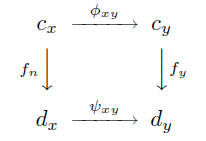
\includegraphics[width=0.3\linewidth]{figures/tda5-1.png}
% 		\label{fig:tda5-1}
% 	\end{figure}
% \end{defn}

% Although we do not have a classification theorem for $\mathbb{R}$-persistence abelian groups, which would then provide a summary of the behavior of the homology of all the complexes $\Cech(X,\epsilon)$, we do have a classification theorem for a subcategory of the category of $\mathbb{N}$-persistence $F$-vector spaces, where $F$ is a field. 

% From the $\mathbb{R}$-persistence simplicial complexes, we just need any partial order preserving map $\mathbb{N} \to \mathbb{R}$ to obtain an $\mathbb{N}-$persistence simplicial complex. Then we can use the classification theorem. 

% There are at least two useful ways to construct such maps. 

% The summary of the methodology is as follows:
% \begin{enumerate}
% 	\item Construct the $\mathbb{R}$-persistence simplicial complex using Cech, Vietoris-
% 	Rips, or witness methods. We will denote it by $\phi$.
% 	\item Select a partial order preserving map $f: \mathbb{N} \to \mathbb{R}$.
% 	\item Construct the associated N-persistence simplicial complex.
% 	\item Construct the associated N-persistence chain complex with coefficients
% 	in F. (It is evident from the finiteness hypotheses on X and
% 	the nature of the constructions that the associated N-persistence F-vector
% 	spaces are tame.)
% 	\item Compute the barcodes associated to the N-persistence F-vector spaces
% \end{enumerate}

\section{Commonly used complexes}

\begin{defn}[\v{C}ech complex]
	For any subset $V\subseteq X$ for which $X = \bigcup_{v\in V}B_\epsilon(v)$, one can construct the nerve of the covering $\{B_\epsilon(v)\}_{v\in V}$. This construction is referred to as the \underline{``\v{C}ech complex"} attached to $V$ and is denoted as $\Cech(V,\epsilon)$.
\end{defn}

\begin{thm}
Let $M$ be a compact Riemannian manifold. Then there is a positive number $e$ so that $\Cech(M, \epsilon)$ is homotopy equivalent to $M$ whenever $\epsilon \leq e$. Moreover, for every $ \epsilon \leq e$, there is a finite subset $V \subseteq M$ so that the subcomplex of $\Cech(V,\epsilon) \subseteq \Cech(M, \epsilon)$ is also homotopy equivalent to $M$.
\end{thm}

However, this construction is computationally expensive. A solution is to construct a simplicial complex which can be recovered solely from the edge information, which motivates the following construction known as the ``Vietoris-Rips complex." 

\begin{defn}[Vietoris-Rips complex]
	Let $X$ be a metric space with metric $d$. Then the  \underline{Vietoris-Rips complex} for $X$, attached to the parameter $\epsilon$, denoted by $VR(X,\epsilon)$, will be the simplicial complex whose vertex set is $X$, and where $\{x_0,\dots, x_k\}$ spans a $k$-simplex if and only if $d(x_i,x_j) \leq \epsilon$ for all $0\leq i,j\leq k.$
\end{defn}

\begin{prop}
	Comparing the \v{C}ech complex and the VR compelx:
	$$ \Cech(X,\epsilon) \subseteq VR (X,2\epsilon) \subseteq \Cech(X,2\epsilon).$$
\end{prop}

However, even the VR complex is computationally expensive. A solution, again, is to use the Voronoi decomposition which studies the subspaces of Euclidean space. 

\begin{thm}[Voronoi decomposition]
	Let $X$ be any metric space, and let $\mathcal{L}\subseteq X$ be a subset (called the set of \textit{landmark points}). Given $\lambda \in \mathcal{L}$, we define the \textit{Voronoi cell} associated to $\lambda, V_\lambda$, by
	$$V_\lambda = \{x\in X| d(x,\lambda) \leq d(x,\lambda^\prime)\} \forall \lambda^\prime \in \mathcal{L}.$$
\end{thm}


\begin{defn}[Delaunay complex]
	Similar to how we define the \v{C}ech complex above, we define the \underline{Delaunay complex} attached to $\mathcal{L}$ to be the nerve of this covering.
\end{defn}

However, for finite metric spaces, the Delaunay complex generically produces degenerate (i.e. discrete) complexes with no $1$-simplices. To solve this, we modify the definition to accommodate pairs of points which are ``almost" equidistant from a pair of landmark points. We thus have the definition below: 

\begin{defn}[Strong witness complex]
	Let X be any metric space, and suppose we are given a finite set $\mathcal{L}$ of points in $X$ (called the landmark set), and a parameter $\epsilon> 0$. For every point $x \in X$, we let $m_x$ denote the distance from this point to the set $\mathcal{L}$, i.e., the minimum distance from $x$ to any point in the landmark set.
	
	Then we define the \underline{strong witness complex} attached to this data to be the complex $W^s(X,\mathcal{L}, \epsilon)$ whose vertex set is $\mathcal{L}$, and where a collection $\{l_0, \dots, l_k\}$ spans a $k$-simplex if and only if there is a point $x \in X$ (the witness) so that $d(x, l_i)\leq m_x + \epsilon$ for all $i$. 
	
	We can also consider the version of this complex in which the $1$-simplices are identical to those of $W(X,\mathcal{L},\epsilon)$, but where the family $\{l_0, \dots, l_k\}$ spans a $k$-simplex if and only if all the pairs $(l_i, l_j)$ are $1$-simplices. We will denote this by $W^s_{VR}$.
\end{defn}

A modified version of the strong witness complex is also useful:

\begin{defn}[Weak witness complex]
	We construct the \underline{weak witness complex}, $W^w(X,\mathcal{L}, \epsilon)$, attached to the given data by declaring that a family $\Lambda = \{l_0, \dots, l_k\}$ spans a $k$-simplex if and only if $\Lambda$ and all its faces admit $\epsilon$ weak witnesses. 
	
	Similar to the definition for strong witness complex, we can also consider the version of the weak witness complex in which the $1$-simplices are identical to those of $W(X,\mathcal{L},\epsilon)$, but where the family $\{l_0, \dots, l_k\}$ spans a $k$-simplex if and only if all the pairs $(l_i, l_j)$ are $1$-simplices. We will denote this by $W^w_{VR}$.
\end{defn}
\chapter{Distances} 
\label{chapter4-distances}

\section{Introduction}

In (\cite{memoli_comparing_2004}), four main categories of data analysis technique for high-dimensional data are compared, which are dimension reduction, clustering, regression analysis, and topological data analysis (TDA). Regarding choosing the appropriate distance in these methods, the paper (\cite{goos_surprising_2001}) examined the commonly used $L_p$ norm and showed that in high dimensional space, whether the notion of distance is qualitatively meaningful depends on the value of $p$.

In TDA, the relevant distance metric include the Gromov-Hausdorff distance, and on the space of persitence diagrams, the Bottleneck distance and the $p$-Wasserstein distance. In our application, we  followed closely the algorithm proposed in (\cite{kerber_geometry_2016}) to compute the $p$-Wasserstein distance between persistence diagrams. 

In this chapter, we will explain in detail the definitions and use cases of the above-mentioned distance metrics. The main references for this chapter are (\cite{chazal_introduction_2021}) and (\cite{phillips_notes}).

\begin{defn}[Metric Spaces]
Given a set $X$ and a function $d: X \times X \to \RR$, we say that the pair $\mathcal{M} = (X,d)$ is a \underline{metric space} on $X$ if and only if $d$ satisfies the following properties:

\begin{enumerate}
\item (Non-negativeness) For all $ x, y \in X, d (x, y) \geq 0.$
    \item (Identity) For all $ x, y \in X, d(x, y) = 0 \iff x = y.$
    \item (Symmetry) For all $x,y\in X, d(x, y) = d(y, x).$
    \item (Triangle Inequality) For all $x,y,z\in X, d(x, z) \leq d(x, y) + d(y, z)$.
\end{enumerate}

A point cloud is essentially a metric space $X$. Elements of $X$ are called points of the metric space. $d(x, y)$ refers to the distance between points $x$ and $y$. 
\end{defn}

\section{Distance between points in $\RR^d$}

\subsection{$L_p$ distance (Minkowski distance)}
\begin{defn}[$L_p$ distance]
Suppose $x, y \in \RR^d.$ Then the $L_p$ distance is defined as 
\begin{align}
    d_p(x,y) = \|x - y\|_p = \left(\sum_{i=1}^d(|a_i - b_i|^p)\right)^{1/p}.
\end{align}
\end{defn}

The following distance metrics are special instances of the $L_p$ distance. 

\begin{defn}[$L_2$ distance (Euclidean distance)]
The most common distance metric is the $L_2$ distance (or Euclidean distance). 
\begin{align}
      d_2(x,y) = \|x - y\|_2 = \left(\sum_{i=1}^d(|a_i - b_i|^2)\right)^{1/2}.
\end{align}
\end{defn}

\begin{defn}[$L_1$ distance (Manhattan distance)]
\begin{align}
      d_1(x,y) = \|x - y\|_1 = \sum_{i=1}^d(|a_i - b_i|).  
\end{align}
\end{defn}

Based on the paper (\cite{goos_surprising_2001}), in metric spaces with a high dimension, the $L_1$ distance and $L_p$ distance with fractional $p$ are more useful than the common $L_2$ distance. For this reason, in many computer vision tasks, the  $L_1$ distance is usually preferred. 

\begin{defn}[$L_\infty$ distance]
\begin{align}
      d_\infty(x,y) = \|x - y\|_\infty = \max_{i=1}^d |a_i - b_i|.
\end{align}
\end{defn}

The following figure compares the above instances of $L_p$ distance:
    \begin{figure}[H]
        \centering
            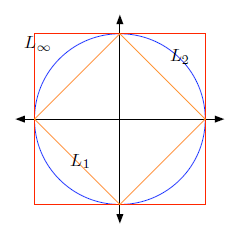
\includegraphics[width=0.5\textwidth]{figures/Lp-distances.png}
            \caption{Comparing the different $L_p$ distances. Adapted from (\cite{phillips_notes}).}
    \end{figure}

\subsection{Cosine distance}
The cosine distance measures the cosine of the angle between vectors $x,y\in \RR^d$
\begin{align}
    d_{cos}(x,y) = \frac{\xx \cdot \yy}{\|\xx\| \|\yy\|} = \frac{\sum_{i =1}^n x_i y_i}{\sqrt{\sum_{i =1}^n x_i^2} \sqrt{\sum_{i =1}^n y_i^2}}
\end{align}

\section{Distance between closed sets of points}

\begin{defn}[$\epsilon$-thickening]
Given a metric space $X$, the set of closed sets of $X$ supports a metric, the Hausdorff metric.

If $A$ is a set in $X$ and $\epsilon > 0$, we define the $\epsilon$-thickening of $A$ to be the set $A^{(\epsilon)}$ defined by

\begin{align}
    A^{(\epsilon)} =\bigcup_{x\in A} B_x(\epsilon),
\end{align}

where $B_x(\epsilon)$ is the open ball of radius $\epsilon$ centered at $x$. 
\end{defn}

\begin{defn}[Hausdorff distance]
    Suppose $A, B \subseteq X$ are closed sets, define their Hausdorff distance $d_H(A, B)$:
    
    \begin{align}
        d_H(A, B) =\inf\{\epsilon >0 \mid A\subseteq B^\epsilon \text{ and } B\subseteq A^\epsilon\}.
    \end{align}
\end{defn}

\begin{defn}[Gromov-Hausdorff distance]
The Gromov-Hausdorff distance extends the Hausdorff distance from subsets of the same metric space to subsets of distinct metric spaces.

Suppose $A, B$ are two closed metric spaces. Then the Gromov-Hausdorff distance is 
    \begin{align}
        d_{GH}(A,B) =\inf_{f,g}\{d_H(f_{A\to X}(A), g_{B\to X}(B))\},
    \end{align}
where $f_{A\to X}$ denotes an isometric embedding of $A$ into some metric space $X$ and $f_{B\to X}$ denotes an isometric embedding of $B$ into some metric space $X$. The infimum is taken over all possible such embeddings. 
\end{defn}

\section{Distance between persistence diagrams}
To make use of the topological features obtained from persistent homology, we need a distance metric to compare persistence diagrams. (\cite{kerber_geometry_2016})

\begin{defn}[Matching between persistent diagrams]
A matching between a pair of persistence diagrams $\dgm_1$ and $\dgm_2$ is a subset $M\subseteq \dgm_1 \times \dgm_2$ such that every point in $\dgm_1 $ and $\dgm_2$ appears exactly once in $M$. That is, for any $x\in \dgm_1$ and $y \in \dgm_2$, $(\{x\} \times \dgm_2) \cap M$ and $(\dgm_1 \times \{y\}) \cap M$ each contains a single pair. A matching is
perfect if every vertex is matched, that is, the matching is a bijection $\eta: \dgm_1 \to \dgm_2$. A perfect matching is illustrated in Figure \ref{fig:perfect-matching} below.
\end{defn}

The above definition has an equivalent formulation as an assignment problem:

\begin{defn}[Matching as assignment problem]
Given a weighted bipartite graph $G = (A \sqcup B,E,w)$, with $|A| = n = |B|$ and a weight function $w : E \to \RR_+$, a matching is a subset $M \subseteq E$ such that every vertex of $A$ and of $B$ is incident to at most one edge in $M$. 
\end{defn}
 
\begin{defn}[Bottleneck distance between persistent diagrams]
The \underline{Bottleneck distance} between a pair of persistence diagrams $\dgm_1$ and $\dgm_2$ is defined by
\begin{align}
    d_B(dgm_1, dgm_2) = \inf_M\{\max_{(x,y)\in M} \|x-y\|_\infty\},
\end{align}
where the infimum is taken over all possible matchings $M$.

If the matching is perfect, then the \underline{Bottleneck distance} can also be expressed as 
\begin{align}
    d_B(dgm_1, dgm2) = \inf_{\eta: \dgm_1 \to \dgm_2}\{\sup_{x\in\dgm_1} \|x-\eta(x)\|_\infty\},
\end{align}
\end{defn}

   \begin{figure}[H]
   \label{matching}
        \centering 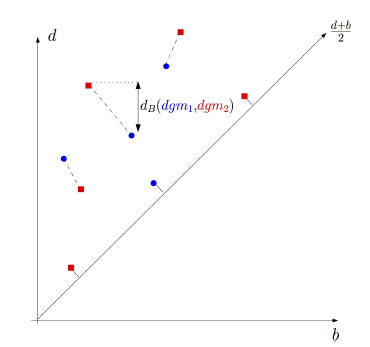
\includegraphics[width=0.5\textwidth]{figures/matching.png}
            \caption{A perfect matching and the Bottleneck distance between the blue and red persistent diagrams. Some points are matched to points on the diagonal. Adapted from (\cite{chazal_introduction_2021}).} \label{fig:perfect-matching}
    \end{figure}
 
\begin{defn}[$p$-Wasserstein distance between persistent diagrams]

Given $p\geq 1$, the $p$-Wasserstein distance between a pair of persistence diagrams $\dgm_1$ and $\dgm_2$ is defined by 
\begin{align}
    W_p(\dgm_1, \dgm_2) = \left(\inf_M \sum_{(x,y)\in M}\|x-y\|^p_\infty\right)^{1/p},
\end{align}
where the infimum is taken over all possible matchings $M$.
If the matching perfect, then the $p$-Wasserstein distance can also be expressed as 
\begin{align}
    W_p(\dgm_1, \dgm_2) = \left(\inf_{\eta: \dgm_1 \to \dgm_2} \sum_{x \in \dgm_1}\|x-\eta(x)\|^p_\infty\right)^{1/p},
\end{align}
As $p$ tends to infinity, the Wasserstein distance approaches
the bottleneck distance.

Note that in this report, when we use the term "Wasserstein distance" interchangably with "$p$-Wasserstein distance."
\end{defn}
\begin{defn}[$q$-tame persistence module]
A persistence module $\VV$ indexed by $T\subseteq \RR$ is $q$-tame if for any $r<s$ in $T$, the rank of the linear map $v^r_s: V_r\to V_s$ is finite.
\end{defn}

\begin{thm}[\cite{chazal_proximity_2009}]
If $\VV$ is a $q$-tame persistence module, then it has a well-defined persistence diagram. 
\end{thm}

\begin{thm}[Stability of persistence diagrams]
Let $\VV$ and $\WW$ 
be two $q$-tame persistence modules. If $\VV$ and $\WW$ are $\delta$-interleaved for some $\delta \geq 0$, then 
\begin{align}
    d_B(\dgm(\VV),\dgm(\WW)) \leq \delta,
\end{align}
\begin{align}
    W_p(\dgm(\VV),\dgm(\WW)) \leq \delta.
\end{align}
\end{thm}

Intuitively, the stability of persistence diagrams means that small perturbations in the persistence module will result in small perturbations in the Bottleneck distance and the $p$-Wasserstein distance between their respective persistence diagrams.

% \section{Comparing the different distances}
% This paper compares the four main categories of data analysis technique for high-dimensional data, each of which either defines or uses the distance metric differently:
% Dimension Reduction
% Clustering
% Regression analysis 
% Topological Data Analysis

\chapter{Dimensionality Reduction} 
\label{chapter2-diffmap}

Diffusion map is one of the common dimensionality reduction methods. This chapter gives an overview of the main ideas and steps in diffusion map. The main references for this chapter are (\cite{coifman_geometric_2005}) and (\cite{coifman_diffusion_2006}).

\section{Key ideas of diffusion map}

\begin{itemize}
    \item The similarity kernel gives us the \textit{local} geometry. As the time steps move forward, we integrate the local geometry and thus reveal the geometric structures at different scales. 
    \item A cluster from a random walk is a region where the probability of escaping this region is low.
\end{itemize}

\section{Main steps of diffusion map}
Now, we summarize the main steps of diffusion maps:
\begin{enumerate}
    \item Construct weighted graph using Gaussian similarity kernel. Each entry in the similarity matrix, $W_{i j}$, is the pairwise similarity value between inputs $i$ and $j$ and is taken as the weight of the edge between nodes $i$ and $j$. 
    
    \begin{align}
        W_{i j } = \exp\{-\frac{\|x_i - x_j\|^2}{2\sigma^2}\}.
    \end{align}
    
    \item We can construct a lazy random walk with the probability of reaching node $j$ from $i$, $p(j \mid i)$, proportional to their pairwise similarity value $W_{i j}$. (The random walk is lazy if we allow $p(i\mid i) > 0$, i.e., to stay at some point $i$ as the time step moves forward). 
    \begin{align}
        p(j\mid i) = \frac{W_{i j}}{\sum_{k} W_{i k}}.
    \end{align}
    
    The probabilities can be represented by a Markov matrix $M$, which is essentially the similarity matrix normalized to have row sums equal to $1$:
     \begin{align}
        M = D^{-1} W, \text{where } D_{i i} =\sum_{k}W_{i k}.
    \end{align}
    The probability of reaching node $j$ from $i$ after $t$ steps is then
    \begin{align}
        p(t,j\mid i) = e_i^T M^t e_j.
    \end{align}

    \item Eigendecomposition of the Markov matrix:
    
    The eigendecomposition of $M$ is derived from the eigendecomposition of $M_s = D^{1/2} M D^{-1/2} = \Omega \Lambda \Omega^T$:
    \begin{align}
        M = D^{-1/2}  \Omega \Lambda \Omega^T D^{-1/2} \coloneqq \Psi \Lambda \Phi^T,
    \end{align}
    
    Note that since $\Psi$ and $\Phi$ are mutually orthogonal, $\Psi$ contains the right eigenvectors, as shown below:
     \begin{align}
        M \Psi =  \Psi \Lambda \Phi^T \Psi = \Psi \Lambda =  \Lambda \Psi.
    \end{align}
    
    The eigendecomposition of $M$ after $t$ steps is then
    \begin{align}
        M = \Psi \Lambda^t \Phi^T.
    \end{align}
    
    \begin{itemize}
        \item Diffusion coordinate functions: right eigenvectors of Markov matrix scaled by their corresponding eigenvalues: 
        \begin{align}
            \Upsilon \coloneqq \Psi \Lambda.
        \end{align}
        \item Diffusion distance after $t$ steps: 
       \begin{align}
            \| e_i^T  \Upsilon - e_j^T \Upsilon  \|^2 = \sum_{k} (p(t,k\mid i) - p(t,k\mid j))^2 (D_{k k}^{-1}).
       \end{align}
       
       \item Growth of eigenvalues leads to geometric properties (more on spectral geometry).
       
       Two extreme situations:
       \begin{enumerate}
           \item If disconnected graph (none of the nodes are connected), then:
           \[P = I, \lambda_i = \lambda_j \quad \forall i, j, \]
           which implies a flat spectrum with zero decay rate.
           \item If fully connected graph (each of the node is connected to all the rest of the nodes), assuming weights of all edges are $1$, then:
            \[\lambda_1 = 1, \lambda_i = 0 \quad \forall i \neq 1.\]
       \end{enumerate}
    \end{itemize}
\end{enumerate}
\chapter{Application to Neural Spiking Data} 
\label{chapter5-application}

\section{Outline of Methods}
We applied the theory outlined in the previous chapters to neural spiking data in which we quantified the pairwise similarity of the neural population responses to different stimuli (each represented as a high-dimensional point cloud) in terms of their geometric and topological structure. The approach of this project was to first embed the data into a lower-dimensional manifold using diffusion map and then apply the method of persistent homology to extract the topological features, specifically the persistence diagrams and the persistence barcodes. In the end, we computed the pairwise Wasserstein distance between the persistence diagrams, which measures the pairwise similarity we set out to find. 

The following flowchart shows a schematic summary of our approach.

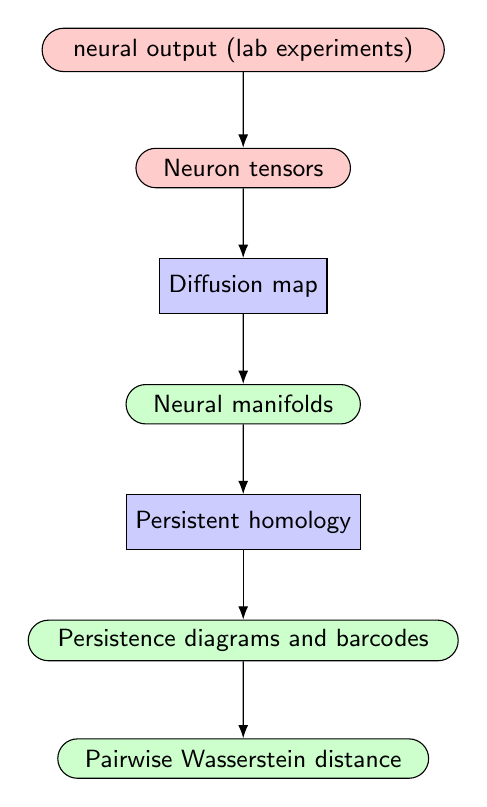
\begin{tikzpicture}[font={\sf \small}]
 \def\smbwd{2cm}
%   \node (BNN) at (-3,0.5) [draw, terminal, minimum width=\smbwd,  fill=yellow!20, minimum height=0.5cm] {Biological Neural Networks}; 
%   \node (ANN) at (2.7,0.5) [draw, terminal, minimum width=\smbwd,  fill=yellow!20, minimum height=0.5cm] {Artificial Neural Networks}; 
  %------------
  \node (experimental) at (0,-0.5) [draw, terminal, minimum width=\smbwd,  fill=red!20, minimum height=0.5cm]{neural output (lab experiments)};
%   \node (artificial) at (2.7,-1)[draw, terminal,minimum width=\smbwd,  fill=red!20, minimum height=0.5cm]{neuron output (simulations)};
  %------------
  \node (tensors) at (0,-2) [draw, terminal, minimum width=\smbwd,  fill=red!20, minimum height=0.5cm] {Neuron tensors}; 
  %------------
  
  \node (diffusion) at (0,-3.5) [draw, process, minimum width=\smbwd, fill=blue!20, minimum height=0.7cm] {Diffusion map};
  %------------
  
  \node (manifolds) at (0,-5) [draw, terminal, minimum width=\smbwd,  fill=green!20, minimum height=0.5cm] {Neural manifolds};
  
   \node (persistent) at (0,-6.5) [draw, process, minimum width=\smbwd, fill=blue!20, minimum height=0.7cm] {Persistent homology};
   
   \node (features) at (0,-8) [draw, terminal, minimum width=\smbwd,  fill=green!20, minimum height=0.5cm] {Persistence diagrams and barcodes};
   
   \node (wasserstein) at (0,-9.5) [draw, terminal, minimum width=\smbwd,  fill=green!20, minimum height=0.5cm] {Pairwise Wasserstein distance};
  
  %------------
  
%  \path [line](BNN) -- (experimental);
%  \path [line](ANN) -- (artificial);
 \path [line](tensors) -- (diffusion);
 \path [line](experimental) -- (tensors) ;
%  \path [line] (artificial) -- (tensors) ;
 \path [line](diffusion) -- (manifolds);
  \path [line](manifolds) -- (persistent);
   \path [line](persistent) -- (features);
  \path [line](features) -- (wasserstein); 
 \end{tikzpicture}
 
\section{Data Collection}

The neural spiking data were collected from lab experiments conducted on mice. The experimental setup is shown in the figure below. Visual stimuli of moving artificial gratings of six different types were flashed in front of the mouse. Each visual stimuli were moving in eight directions. Neuron output of the mouse retina was recorded with electrodes and encoded in peristimulus (PSTH) diagrams. Each PSTH diagram shows the firing rate of one neuron over time for each of the eight directions respectively. Brighter pixels indicate higher firing rates.
 \begin{figure}[H]
        \centering
            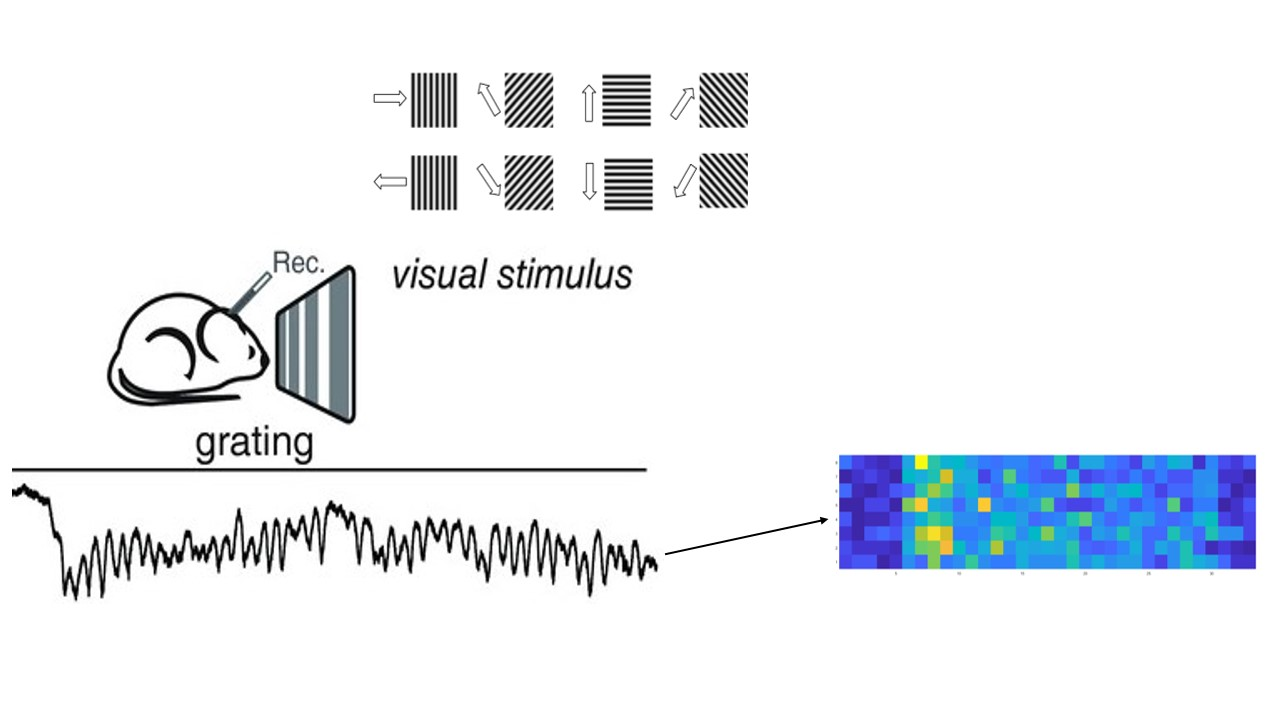
\includegraphics[width=0.55\textwidth]{figures/Slide5.jpg}
            \caption{Visualising neural data from lab experiments.}
    \end{figure}
    
\begin{defn}[Neural population response]
    Suppose $\mathcal{S}$ is a set of $S$ visual stimuli (e.g., images) $\mathcal{S} = \{s_1, s_2,\dots, s_S\}$, each having $T$ number of shifts (which is equivalent to the number of pixels in the PSTH diagrams in this application).
    
    The \underline{neural population response} of a set of $N$ neurons to a stimulus $m_i$ over all transformations is $\mathcal{N} = \{\vec{n}_1, \vec{n}_2, \dots, \vec{n}_N\},$ where $\vec{n}_i \in \mathbb{R}^T$. 
\end{defn}

\begin{defn}[Neural tensors]
    Each \underline{neural tensor} encodes the neural population response of a set of neurons to a set of stimulus over all transformations. It is thus a $3$-way tensor of dimension $N$-by-$S$-by-$T$.
\end{defn} 

The neural spiking data set used in this project is represented by a $3$-way tensor of dimension $698$-by-$6$-by-$264$. The three dimensions represent the following respectively: there are in total $698$ neurons $6$, $6$ types of visual stimuli, and $264$ number of pixels in the PSTH diagram.

With this neural spiking data set, we can create six point clouds, each corresponds to the neural population response towards one type of stimuli, which we denote as $X_1, X_2, \dots,X_6$. Each of the point cloud $X_i$ is thus represented by a matrix of dimension $698$-by-$264$, giving us a point cloud of $698$ points in $\RR^{264}$. 

\section{Step 1: Dimensionality Reduction}

The main motivation behind dimensionality reduction is that the intrinsic dimension of the data is usually much lower than the extrinsic dimension and the high-dimensionality is usually just an artifact of the representation. The representation of data has a potentially large degree of freedom, that is, the number of variables that are really necessary to describe the data is much smaller.

The Manifold Hypothesis states that real-world high-dimensional data lie on low-dimensional manifolds embedded within the high-dimensional space. (\cite{deepai_2019})

% main idea behind manifold learning:
In the context of neuroscience, neural spiking data is high-dimensional, but the neural connections constrain the possible patterns of population activity (\cite{okun_diverse_2015}, \cite{sadtler_neural_2014}, \cite{tsodyks_attractor_1999}) and that the possible patterns are confined to a low-dimensional manifold (\cite{stopfer_intensity_2003},  \cite{yu_gaussian-process_2009}) spanned by a few independent patterns that are called ``neural modes." (\cite{gallego_neural_2017})

In terms of implementation, we used the pydiffmap package (\cite{eastman_pydiffmap_2017}). In our implementation, we reduced the dimensionaltity of each point cloud from the space of $\RR^{264}$ to $\RR^3$ using diffusion map. The resulting three-dimensional embedding of the original point clouds colored by the first three diffusion coordinates are shown below:
\begin{figure}[H]
\centering
\begin{subfigure}[b]{0.3\textwidth}
    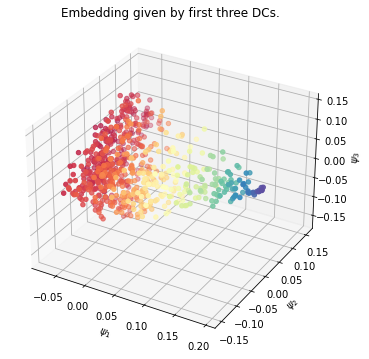
\includegraphics[width=\textwidth]{figures/X1_embedding.png}
    \caption{Three-dimensional embedding of the original point cloud $X_1$.}
\end{subfigure}
\hfill
\begin{subfigure}[b]{0.3\textwidth}
    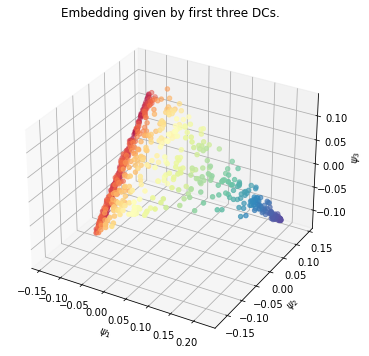
\includegraphics[width=\textwidth]{figures/X2_embedding.png}
    \caption{Three-dimensional embedding of the original point cloud $X_2$.}
\end{subfigure}
\hfill
\begin{subfigure}[b]{0.3\textwidth}
    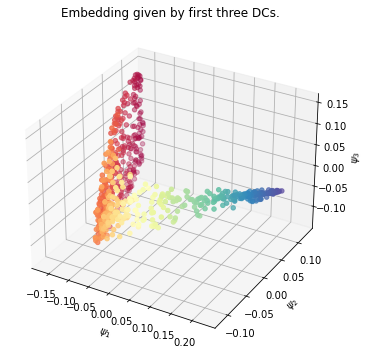
\includegraphics[width=\textwidth]{figures/X3_embedding.png}
    \caption{Three-dimensional embedding of the original point cloud $X_3$.}
\end{subfigure}
\hfill
\begin{subfigure}[b]{0.3\textwidth}
    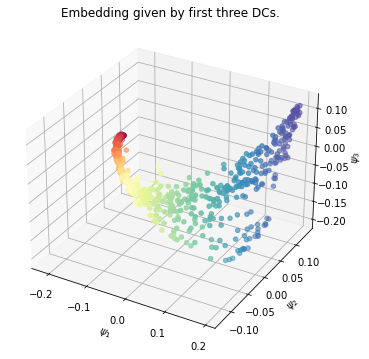
\includegraphics[width=\textwidth]{figures/X4_embedding.png}
    \caption{Three-dimensional embedding of the original point cloud $X_4$.}
\end{subfigure}
\hfill
\begin{subfigure}[b]{0.3\textwidth}
    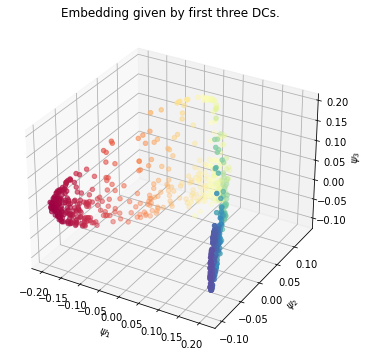
\includegraphics[width=\textwidth]{figures/X5_embedding.png}
    \caption{Three-dimensional embedding of the original point cloud $X_5$.}
\end{subfigure}
\hfill
\begin{subfigure}[b]{0.3\textwidth}
    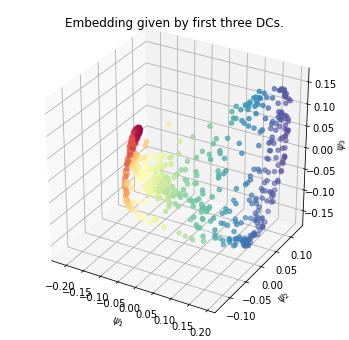
\includegraphics[width=\textwidth]{figures/X6_embedding.png}
    \caption{Three-dimensional embedding of the original point cloud $X_6$.}
\end{subfigure}
\end{figure}

\section{Step 2: Persistent Homology}

Having obtained the three-dimensional embeddings of the point clouds corresponding to six stimuli types, we applied persistent homology to extract the topological features from the six embeddings respectively. In this step, these topological features are represented by persistence barcodes and persistence diagrams.

Our implementation used the package ripser (\cite{ctralie2018ripser}) to obtain the respective persistence diagrams from the embeddings. Using the (birth, death)-intervals from each persistence diagram, we drew the equivalent persistence barcode representation. The complete code can be found in Appendix \ref{AppendixA}. The following figures show the results from applying persistent homology.
\begin{figure}[H]
\centering
\begin{subfigure}[b]{0.2\textwidth}
    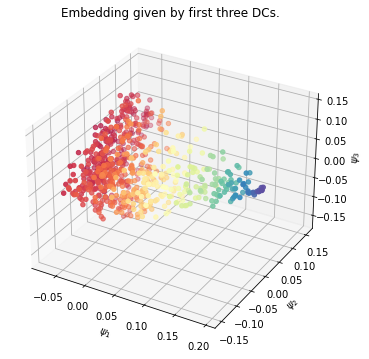
\includegraphics[width=\textwidth]{figures/X1_embedding.png}
    \caption{Three-dimensional embedding of the original point cloud $X_1$.}
\end{subfigure}
\hfill
\begin{subfigure}[b]{0.75\textwidth}
    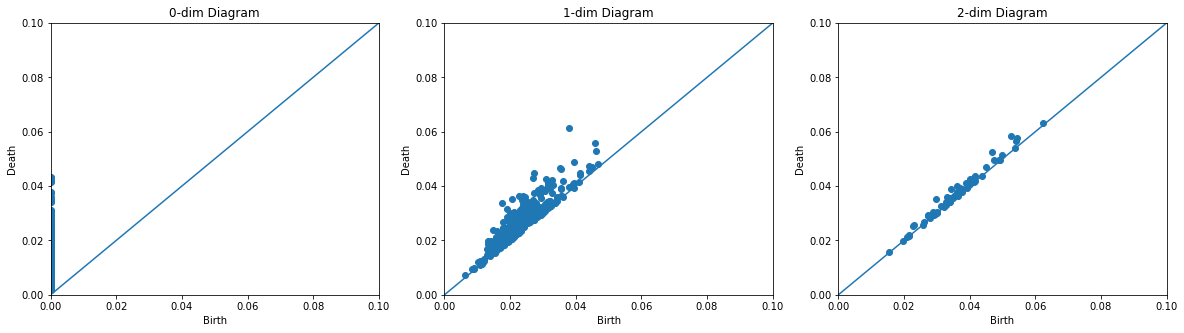
\includegraphics[width=\textwidth]{figures/X1_H0.png}
    \caption{Persistence diagrams.}
\end{subfigure}
\begin{subfigure}[b]{0.25\textwidth}

\includegraphics[width=\textwidth]{figures/white.png} 
\end{subfigure}
\begin{subfigure}[b]{0.24\textwidth}
    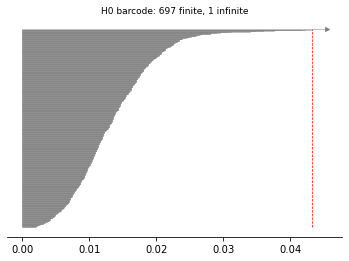
\includegraphics[width=\textwidth]{figures/X1_H0_barcode.png}
    \caption{}
\end{subfigure}
\begin{subfigure}[b]{0.24\textwidth}
    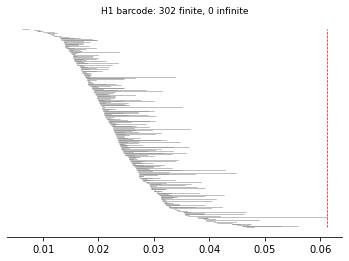
\includegraphics[width=\textwidth]{figures/X1_H1_barcode.png}
        \caption{Persistence barcodes.}
\end{subfigure}
\begin{subfigure}[b]{0.24\textwidth}
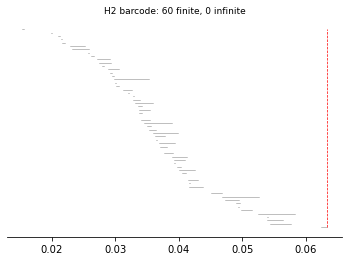
\includegraphics[width=\textwidth]{figures/X1_H2_barcode.png}
 \caption{}
\end{subfigure}
\caption{Results for applying persistent homology on the three-dimensional embedding of $X_1$.}
\end{figure}

\begin{figure}[H]
\centering
\begin{subfigure}[b]{0.2\textwidth}
    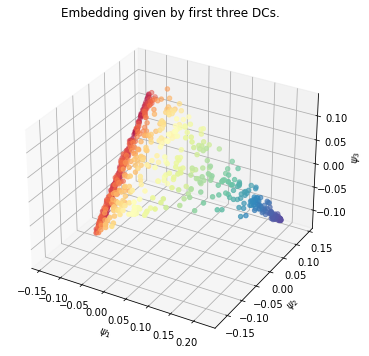
\includegraphics[width=\textwidth]{figures/X2_embedding.png}
    \caption{Three-dimensional embedding of the original point cloud $X_2$.}
\end{subfigure}
\hfill
\begin{subfigure}[b]{0.75\textwidth}
    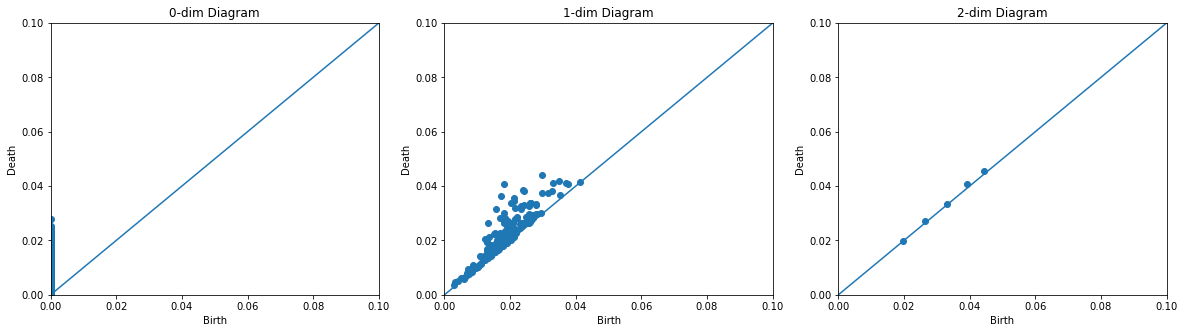
\includegraphics[width=\textwidth]{figures/X2_H0.png}
    \caption{Persistence diagrams.}
\end{subfigure}
\begin{subfigure}[b]{0.25\textwidth}

\includegraphics[width=\textwidth]{figures/white.png} 
\end{subfigure}
\begin{subfigure}[b]{0.24\textwidth}
    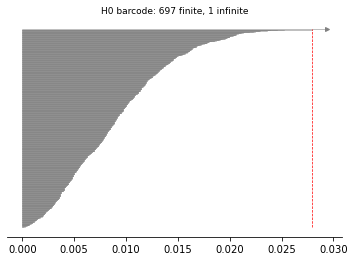
\includegraphics[width=\textwidth]{figures/X2_H0_barcode.png}
    \caption{}
\end{subfigure}
\begin{subfigure}[b]{0.24\textwidth}
    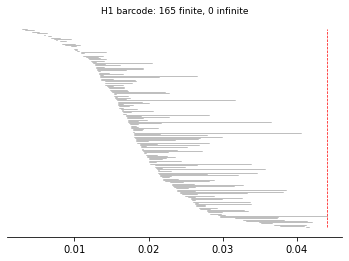
\includegraphics[width=\textwidth]{figures/X2_H1_barcode.png}
        \caption{Persistence barcodes.}
\end{subfigure}
\begin{subfigure}[b]{0.24\textwidth}
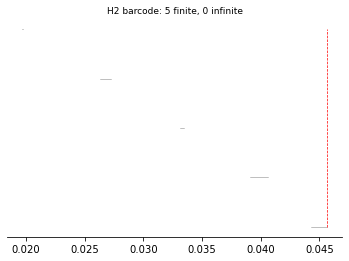
\includegraphics[width=\textwidth]{figures/X2_H2_barcode.png}
 \caption{}
\end{subfigure}
\caption{Results for applying persistent homology on the three-dimensional embedding of $X_2$.}
\end{figure}

\begin{figure}[H]
\centering
\begin{subfigure}[b]{0.2\textwidth}
    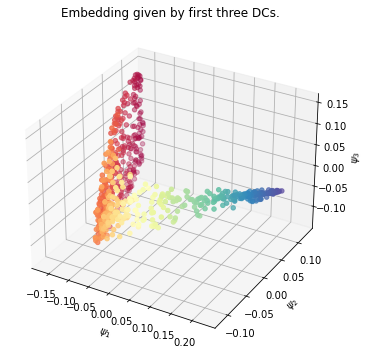
\includegraphics[width=\textwidth]{figures/X3_embedding.png}
    \caption{Three-dimensional embedding of the original point cloud $X_3$.}
\end{subfigure}
\hfill
\begin{subfigure}[b]{0.75\textwidth}
    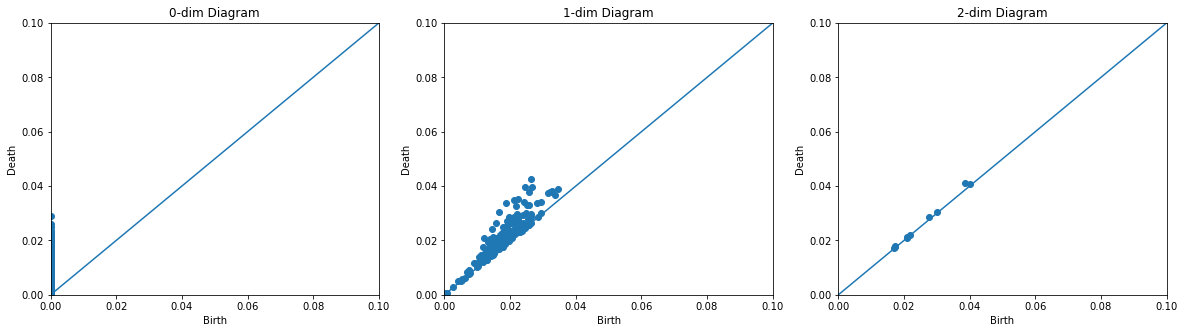
\includegraphics[width=\textwidth]{figures/X3_H0.png}
    \caption{Persistence diagrams.}
\end{subfigure}
\begin{subfigure}[b]{0.25\textwidth}

\includegraphics[width=\textwidth]{figures/white.png} 
\end{subfigure}
\begin{subfigure}[b]{0.24\textwidth}
    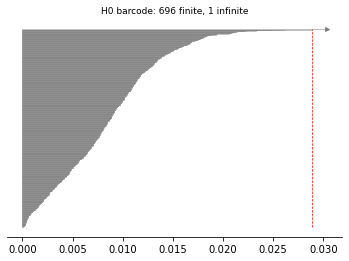
\includegraphics[width=\textwidth]{figures/X3_H0_barcode.png}
    \caption{}
\end{subfigure}
\begin{subfigure}[b]{0.24\textwidth}
    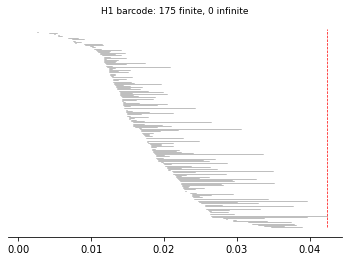
\includegraphics[width=\textwidth]{figures/X3_H1_barcode.png}
        \caption{Persistence barcodes.}
\end{subfigure}
\begin{subfigure}[b]{0.24\textwidth}
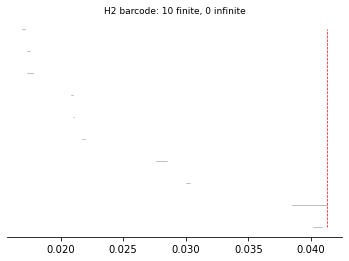
\includegraphics[width=\textwidth]{figures/X3_H2_barcode.png}
 \caption{}
\end{subfigure}
\caption{Results for applying persistent homology on the three-dimensional embedding of $X_3$.}
\end{figure}

\begin{figure}[H]
\centering
\begin{subfigure}[b]{0.2\textwidth}
    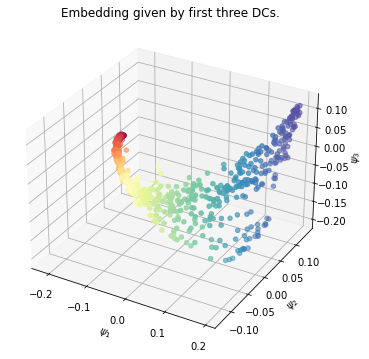
\includegraphics[width=\textwidth]{figures/X4_embedding.png}
    \caption{Three-dimensional embedding of the original point cloud $X_4$.}
\end{subfigure}
\hfill
\begin{subfigure}[b]{0.75\textwidth}
    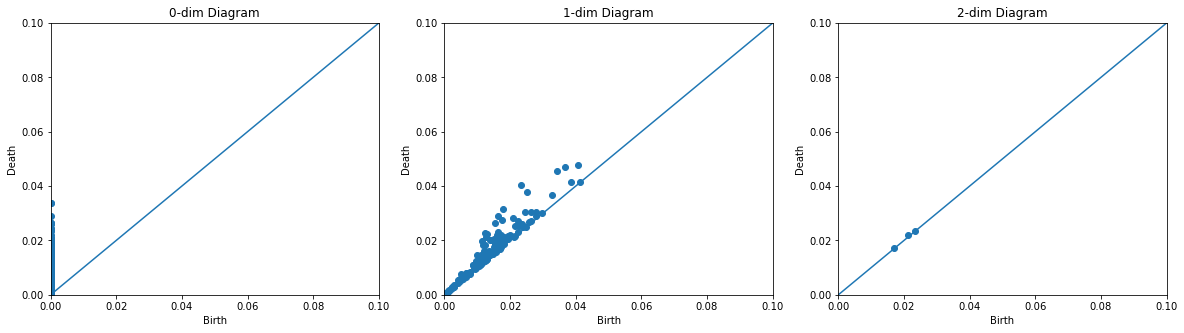
\includegraphics[width=\textwidth]{figures/X4_H0.png}
    \caption{Persistence diagrams.}
\end{subfigure}
\begin{subfigure}[b]{0.25\textwidth}

\includegraphics[width=\textwidth]{figures/white.png} 
\end{subfigure}
\begin{subfigure}[b]{0.24\textwidth}
    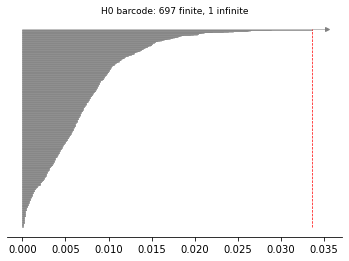
\includegraphics[width=\textwidth]{figures/X4_H0_barcode.png}
    \caption{}
\end{subfigure}
\begin{subfigure}[b]{0.24\textwidth}
    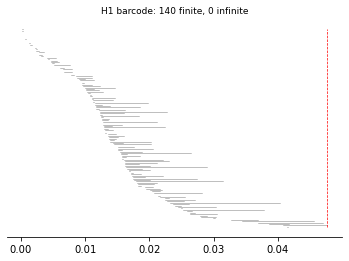
\includegraphics[width=\textwidth]{figures/X4_H1_barcode.png}
        \caption{Persistence barcodes.}
\end{subfigure}
\begin{subfigure}[b]{0.24\textwidth}
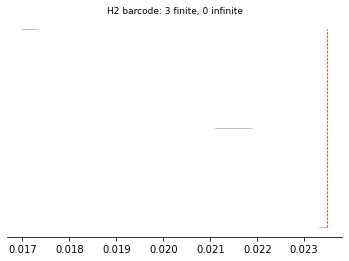
\includegraphics[width=\textwidth]{figures/X4_H2_barcode.png}
 \caption{}
\end{subfigure}
\caption{Results for applying persistent homology on the three-dimensional embedding of $X_4$.}
\end{figure}

\begin{figure}[H]
\centering
\begin{subfigure}[b]{0.2\textwidth}
    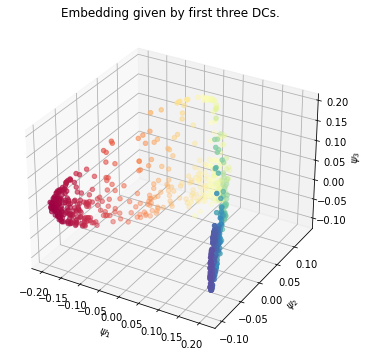
\includegraphics[width=\textwidth]{figures/X5_embedding.png}
    \caption{Three-dimensional embedding of the original point cloud $X_5$.}
\end{subfigure}
\hfill
\begin{subfigure}[b]{0.75\textwidth}
    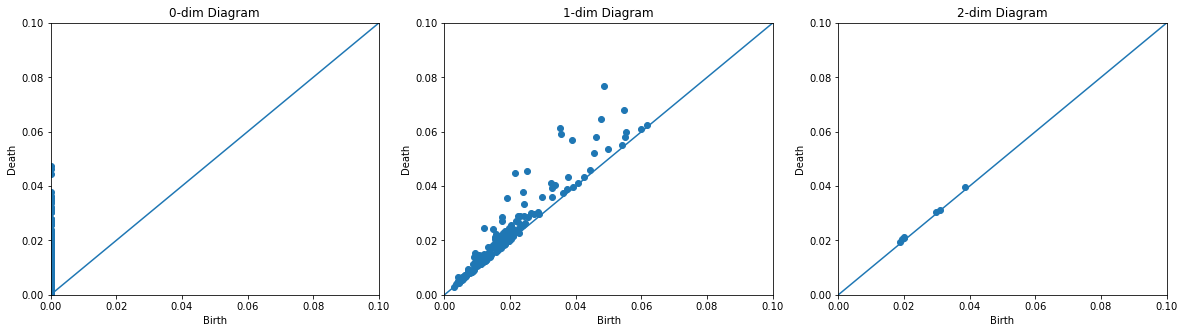
\includegraphics[width=\textwidth]{figures/X5_H0.png}
    \caption{Persistence diagrams.}
\end{subfigure}
\begin{subfigure}[b]{0.25\textwidth}

\includegraphics[width=\textwidth]{figures/white.png} 
\end{subfigure}
\begin{subfigure}[b]{0.24\textwidth}
    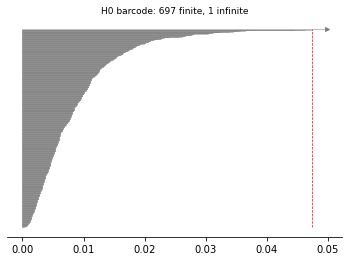
\includegraphics[width=\textwidth]{figures/X5_H0_barcode.png}
    \caption{}
\end{subfigure}
\begin{subfigure}[b]{0.24\textwidth}
    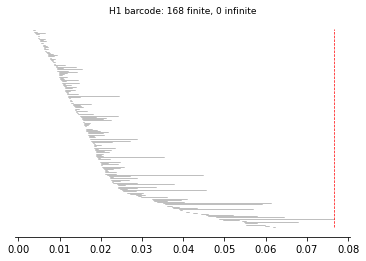
\includegraphics[width=\textwidth]{figures/X5_H1_barcode.png}
        \caption{Persistence barcodes.}
\end{subfigure}
\begin{subfigure}[b]{0.24\textwidth}
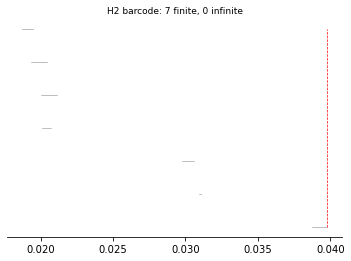
\includegraphics[width=\textwidth]{figures/X5_H2_barcode.png}
 \caption{}
\end{subfigure}
\caption{Results for applying persistent homology on the three-dimensional embedding of $X_5$.}
\end{figure}

\begin{figure}[H]
\centering
\begin{subfigure}[b]{0.2\textwidth}
    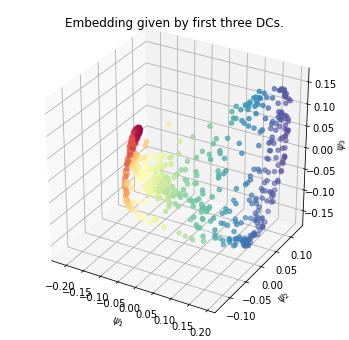
\includegraphics[width=\textwidth]{figures/X6_embedding.png}
    \caption{Three-dimensional embedding of the original point cloud $X_6$.}
\end{subfigure}
\hfill
\begin{subfigure}[b]{0.75\textwidth}
    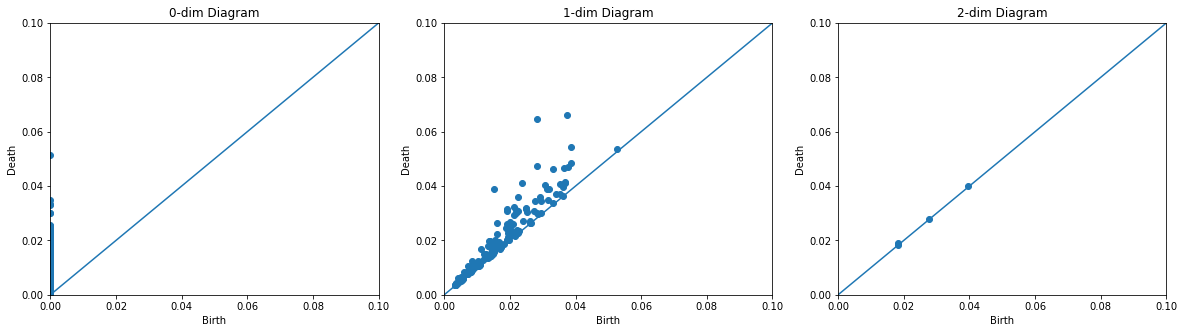
\includegraphics[width=\textwidth]{figures/X6_H0.png}
    \caption{Persistence diagrams.}
\end{subfigure}
\begin{subfigure}[b]{0.25\textwidth}

\includegraphics[width=\textwidth]{figures/white.png} 
\end{subfigure}
\begin{subfigure}[b]{0.24\textwidth}
    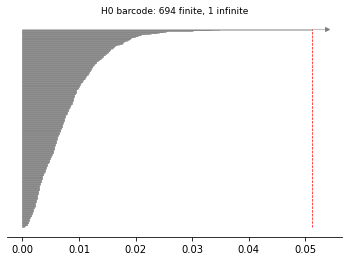
\includegraphics[width=\textwidth]{figures/X6_H0_barcode.png}
    \caption{}
\end{subfigure}
\begin{subfigure}[b]{0.24\textwidth}
    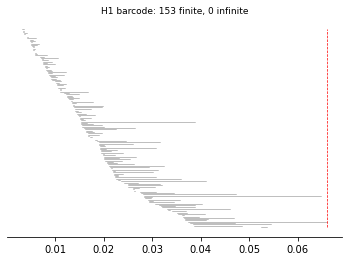
\includegraphics[width=\textwidth]{figures/X6_H1_barcode.png}
        \caption{Persistence barcodes.}
\end{subfigure}
\begin{subfigure}[b]{0.24\textwidth}
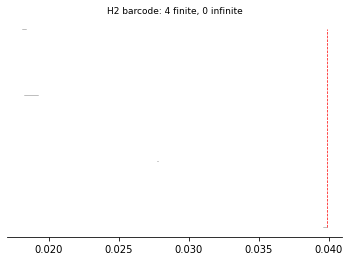
\includegraphics[width=\textwidth]{figures/X6_H2_barcode.png}
 \caption{}
\end{subfigure}
\caption{Results for applying persistent homology on the three-dimensional embedding of $X_6$.}
\end{figure}

\section{Step 3: Pairwise Wasserstein distance}
In the last step, we used the gudhi package (\cite{gudhi:urm}) to compute the pairwise Wasserstein distance between the persistence diagrams. The method used is based on (\cite{kerber_geometry_2016}). 

We first computed the first pairwise distances between the persistence diagrams for each of the six point clouds. 

\begin{table}[!htbp]
        \centering
        \small
        \setlength\tabcolsep{5pt}
        \begin{tabular}{|c|c|c|c|c|c|c|}
\hline
 $H_0$& $X_1$ & $X_2$ & $X_3$ & $X_4$ & $X_5$ & $X_6$\\
 \hline
$X_1$ &
0.0&
2.77&
3.05&
3.95&
3.08&
3.42
\\
\hline
$X_2$ &
2.77&
0.0&
0.43&
1.35&
1.0&
0.84
\\
\hline
$X_3$ &
3.05&
0.43&
0.0&
1.03&
0.94&
0.66
\\
\hline
$X_4$ &
3.95&
1.35&
1.03&
0.0&
1.11&
0.72
\\
\hline
$X_5$ &
3.08&
1.0&
0.94&
1.11&
0.0&
0.51
\\
\hline
$X_6$ &
3.42&
0.84&
0.66&
0.72&
0.51&
0.0
\\
\hline
\end{tabular}
\caption{Pairwise Wasserstein distance between persistent diagrams for homology group $H_0$.}
\label{tab:Wass_H0}
\end{table}

\begin{table}[!htbp]
        \centering
        \small
        \setlength\tabcolsep{5pt}
        \begin{tabular}{|c|c|c|c|c|c|c|}
\hline
 $H_1$& $X_1$ & $X_2$ & $X_3$ & $X_4$ & $X_5$ & $X_6$ \\ \hline
$X_1$ &
0.0&
0.46&
0.5&
0.64&
0.64&
0.55

\\\hline
$X_2$ &
0.46&
0.0&
0.17&
0.29&
0.36&
0.3
\\\hline
$X_3$ &
0.5&
0.17&
0.0&
0.25&
0.33&
0.3
\\\hline 
$X_4$ &
0.64&
0.29&
0.25&
0.0&
0.27&
0.29
\\\hline 
$X_5$ &
0.64&
0.36&
0.33&
0.27&
0.0&
0.26

\\\hline
$X_6$ &
0.55&
0.3&
0.3&
0.29&
0.26&
0.0\\
\hline
\end{tabular}
\caption{Pairwise Wasserstein distance between persistent diagrams for homology group $H_1$.}
\label{tab:Wass_H1}
\end{table}

\begin{table}[!htbp]
        \centering
        \small
        \setlength\tabcolsep{5pt}
        \begin{tabular}{|c|c|c|c|c|c|c|}
\hline
 $H_2$& $X_1$ & $X_2$ & $X_3$ & $X_4$ & $X_5$ & $X_6$ \\ \hline
$X_1$ &
0.0&
0.06&
0.06&
0.06&
0.06&
0.06
\\
\hline
$X_2$ &
0.06&
0.0&
0.01&
0.0&
0.01&
0.0
\\
\hline
$X_3$ &
0.06&
0.01&
0.0&
0.0&
0.01&
0.0
\\
\hline
$X_4$ &
0.06&
0.0&
0.0&
0.0&
0.0&
0.0
\\
\hline
$X_5$ &
0.06&
0.01&
0.01&
0.0&
0.0&
0.0
\\
\hline
$X_6$ &
0.06&
0.0&
0.0&
0.0&
0.0&
0.0
\\
\hline
\end{tabular}
\caption{Pairwise Wasserstein distance between persistent diagrams for homology group $H_2$.}
\label{tab:Wass_H2}
\end{table}

Building upon the same method, we further compared the six point clouds with known three-dimensional shapes ($2$-sphere and torus) based on the Wasserstein distance.

First, we extracted the topological features of the $2$-sphere and three-dimensional torus, as we did for the point clouds in Step 2. 
\begin{figure}[H]
\centering
\begin{subfigure}[b]{0.2\textwidth}
    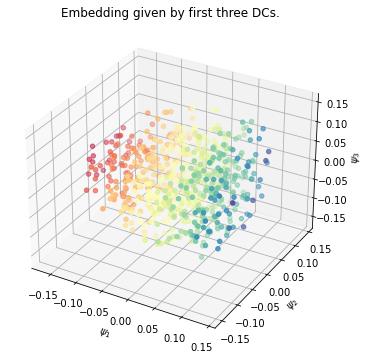
\includegraphics[width=\textwidth]{figures/dsphere.png}
    \caption{Scatter plot for $2$-sphere.}
\end{subfigure}
\hfill
\begin{subfigure}[b]{0.75\textwidth}
    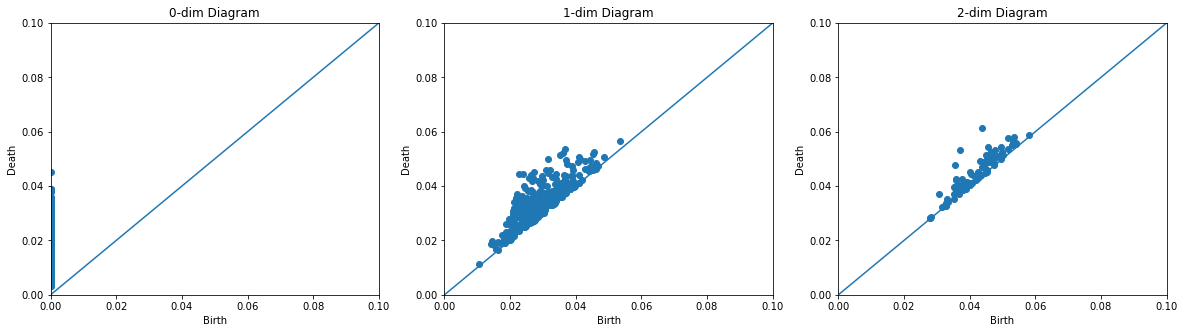
\includegraphics[width=\textwidth]{figures/dsphere_Hk.png}
    \caption{Persistence diagrams.}
\end{subfigure}
\begin{subfigure}[b]{0.25\textwidth}

\includegraphics[width=\textwidth]{figures/white.png} 
\end{subfigure}
\begin{subfigure}[b]{0.24\textwidth}
    \includegraphics[width=\textwidth]{figures/dsphere_H0_barcode.png}
    \caption{}
\end{subfigure}
\begin{subfigure}[b]{0.24\textwidth}
    \includegraphics[width=\textwidth]{figures/dsphere_H1_barcode.png}
        \caption{Persistence barcodes.}
\end{subfigure}
\begin{subfigure}[b]{0.24\textwidth}
\includegraphics[width=\textwidth]{figures/dsphere_H2_barcode.png}
 \caption{}
\end{subfigure}
\caption{Results for applying persistent homology on the $2$-sphere.}
\end{figure}

\begin{figure}[H]
\centering
\begin{subfigure}[b]{0.2\textwidth}
    \includegraphics[width=\textwidth]{figures/torus.png}
    \caption{Scatter plot for the three-dimensional torus.}
\end{subfigure}
\hfill
\begin{subfigure}[b]{0.75\textwidth}
    \includegraphics[width=\textwidth]{figures/torus_Hk.png}
    \caption{Persistence diagrams.}
\end{subfigure}
\begin{subfigure}[b]{0.25\textwidth}
\includegraphics[width=\textwidth]{figures/white.png} 
\end{subfigure}
\begin{subfigure}[b]{0.24\textwidth}
    \includegraphics[width=\textwidth]{figures/torus_H0_barcode.png}
    \caption{}
\end{subfigure}
\begin{subfigure}[b]{0.24\textwidth}
    \includegraphics[width=\textwidth]{figures/torus_H1_barcode.png}
        \caption{Persistence barcodes.}
\end{subfigure}
\begin{subfigure}[b]{0.24\textwidth}
\includegraphics[width=\textwidth]{figures/torus_H2_barcode.png}
 \caption{}
\end{subfigure}
\caption{Results for applying persistent homology on the three-dimensional torus.}
\end{figure}

Then, we computed the Wasserstein distance between the six point clouds and the known shapes:

\begin{table}[!htbp]
        \centering
        \small
        \setlength\tabcolsep{5pt}
        \begin{tabular}{|c|c|c|c|c|c|c|}
\hline
  $H_0$& $X_1$ & $X_2$ & $X_3$ & $X_4$ & $X_5$ & $X_6$ \\ \hline
$2$-sphere & 2.48 & 4.46&  4.64 & 5.18 & 4.53 & 4.83\\\hline
torus & 3.63 &  1.46 & 1.31 & 0.73 & 1.38 & 1.06 \\ \hline
\end{tabular}
\caption{Wasserstein distance between persistent diagrams of the point clouds and $2$-sphere and torus (homology group $H_0$).}
\label{tab:sphere-H0}
\end{table}


\begin{table}[!htbp]
        \centering
        \small
        \setlength\tabcolsep{5pt}
        \begin{tabular}{|c|c|c|c|c|c|c|}
\hline
$H_1$& $X_1$ & $X_2$ & $X_3$ & $X_4$ & $X_5$ & $X_6$ \\ \hline
$2$-sphere & 0.62 &   0.77 & 0.80 & 0.87 & 0.85 & 0.76\\\hline
torus & 0.74 & 0.49 & 0.44 & 0.34 & 0.45 & 0.47\\ \hline
\end{tabular}
\caption{Wasserstein distance between persistent diagrams of the point clouds and $2$-sphere and torus (homology group $H_1$).}
\label{tab:sphere-H1}
\end{table}

\begin{table}[!htbp]
        \centering
        \small
        \setlength\tabcolsep{5pt}
        \begin{tabular}{|c|c|c|c|c|c|c|}
\hline
$H_2$ & $X_1$ & $X_2$ & $X_3$ & $X_4$ & $X_5$ & $X_6$ \\ \hline
$2$-sphere & 0.11 &   0.12 & 0.12 & 0.12 & 0.13 & 0.12\\\hline
torus & 0.057 & 0.017 & 0.018  & 0.016 & 0.018 & 0.016 \\ \hline
\end{tabular}
\caption{Wasserstein distance between persistent diagrams of the point clouds and $2$-sphere and torus (homology group $H_2$).}
\label{tab:sphere-H2}
\end{table}

\section{Analysis of results}
Based on the results from the above tables of Wasserstein distances, our observations and inferences are as follows.

\begin{enumerate}
    \item The topological structure for $X_1$ is distinct from the rest. 
    
    Based on the pairwise Wasserstein distances in Tables \ref{tab:Wass_H0} and \ref{tab:Wass_H1}, $X_1$ is notably different from the rest of the point clouds in terms of topological structure. In the context of our application, this implies that the neural population response evoked by stimulus type 1 is significantly different from the other stimulus types. This observation leads us to hypothesize that there is some neuroscientific reason behind this distinction in the topological structure of neural population response. It might be interesting to conduct further lab experiments to investigate what special properties this stimulus has and why it causes such different  neural population response. 
    
    \item Wasserstein distances between persistence diagrams are nearly negligible for $H_2$.
    
    Based on Table \ref{tab:Wass_H2}, pairwise Wasserstein distances between persistence diagrams for $H_2$ are small enough to be nearly negligible. This implies that the intrinsic dimensionality of this neural data might be even lower than three-dimensional since there is no significant differences in homology groups $H_2$ for the point clouds.
    
    \item Shape comparison with $2$-sphere and torus.
    
    Based on Tables \ref{tab:sphere-H0} and \ref{tab:sphere-H1}, the Wasserstein distances between the point clouds and the $2$-sphere are smaller than the Wasserstein distances between the point clouds and the torus for all $X_i$ except for $X_1$. We can thus infer that except for $X_1$, all other point clouds are more similar to the shape of a torus than the $2$-sphere. This implies that the topological structure of the neural population response evoked by stimuli type 1 is more similar to a sphere while the neural population response evoked by the rest of the stimuli types used in the experiments are more similar to a torus. 
    
    It would be interesting to compare this result with the hypothesis in (\cite{ben-yishai_theory_1995}, \cite{Blumenfeld_2006}, \cite{goldberg_randomized_2004},    \cite{singh_top_v1_2008}):
    If we are given an oriented stimulus, and if the orientation is a circular variable, then the hypothesis is that the neural population response evoked by such stimulus must have a topological structure equivalent to that of a circle. However, to fully test this hypothesis, further experiments with different types of stimuli need to be conducted.
\end{enumerate}

\section{Conclusion}
In this chapter, we demonstrated our proposed approach to compare the point clouds that represent the neural population response to different stimuli. Our proposed approach is contingent on the topological structures of the point clouds.  

One significant limitation in this specific application is that lab data usually involve a lot of sampling errors such as missing data and inconsistent densities, causing noise to the true underlying geometry of the neural population response. Persistent homology works well on synthetic data, but might not work when the sampling errors are too significant.

The advantages of topological approach is that we can provide a succinct and useful summary of the global geometric structure of the neural spiking data, thus obtaining a useful account of how similarly the neurons collectively respond to visual stimuli. This is especially important in applications where the notion of connectedness and clusters are salient. As an emerging field, TDA will certainly see more applications in solving problems that involve understanding the geometric and topological structure of high-dimensional data.

\printbibliography[heading=bibintoc]


\appendix 
% Appendix Template

\chapter{Implementation Code} % Main appendix title

\label{AppendixA} % Change X to a consecutive letter; for referencing this appendix elsewhere, use \ref{AppendixX}
\includepdf[pages=-,pagecommand={},width=\textwidth]{Persistent_Homology_Features_retina_DiffMap+TDA_report.pdf}

\listoftables % Prints the list of tables
\label{lst:tabs}

\listoffigures % Prints the list of figures
\label{lst:figs}

%----------------------------------------------------------------------------------------
%	ABBREVIATIONS
%----------------------------------------------------------------------------------------

% \begin{abbreviations}{ll} % Include a list of abbreviations (a table of two columns)
%
% \textbf{LAH} & \textbf{L}ist \textbf{A}bbreviations \textbf{H}ere\\
% \textbf{WSF} & \textbf{W}hat (it) \textbf{S}tands \textbf{F}or\\
%
% \end{abbreviations}

\end{document}
